\documentclass{../grid-link-report}
\SetClassAssetsDir{../class-assets}

\newcommand{\projectassetsdir}{../project-assets}

\project{Heywood BESS}
\client{Atmos Renewables}
\title{Releasable User Guide - PSCAD}
\docnumber{HEYWOODBESS-GR-RPT-002}
\issueddate{25 July 2025}
\revision{1-1-0}
\revisionhistorycsvpath{report-assets/revision-history.csv}
\clientlogopath{\projectassetsdir/client-logo.jpg}

\usepackage{listings}
\usepackage{tabto}
\usepackage[justification=centering]{caption}%
\usepackage{pgfplotstable} % For reading and displaying tables from CSV files
\usepackage{booktabs}      % For better-looking tables
\usepackage{adjustbox}
\usepackage{float}

\lstset{
	basicstyle=\ttfamily\small,
	breaklines=true,          % Wrap long lines
	breakatwhitespace=false,  % Don't break only at whitespace
	columns=flexible,         % Better wrapping
	frame=single,             % Optional border around code
	captionpos=b              % Caption below (optional)
}



\begin{document}
	% Draft commands
	%\adddraftstamp
	%\listoftodos
	
	\frontmatter
	\maketitle
	
	\makedisclaimer
	\clearpage
	\tableofcontents
	\makerevisionhistorypage
	%\makeaboutgridlink
	
	\mainmatter
	
	\chapter{Introduction}

	\section{Overview of generating station }
	The Heywood Battery Energy Storage System (HEYWOODBESS) is a $\pm~285MW/1140MWh$ Battery Energy Storage Project, is located 5 km from the town of Heywood and 300 km west of Melbourne in Victoria as shown in Figure~\ref{fig:project-location}. The project is expected to connect directly to the existing 275 kV Heywood terminal station via a single high voltage cable.

HEYWOODBESS will include 92 SMA Sunny Central 4.6 MVA (SCS 4600 UP-S) converters which will be connected to two 275/33/33kV, 160MVA three winding transformers through a 33kV reticulation system. Each converter will have a dedicated 33/0.69kV, 4.6 MVA step up transformer.


\begin{figure}[H]
	\centering
	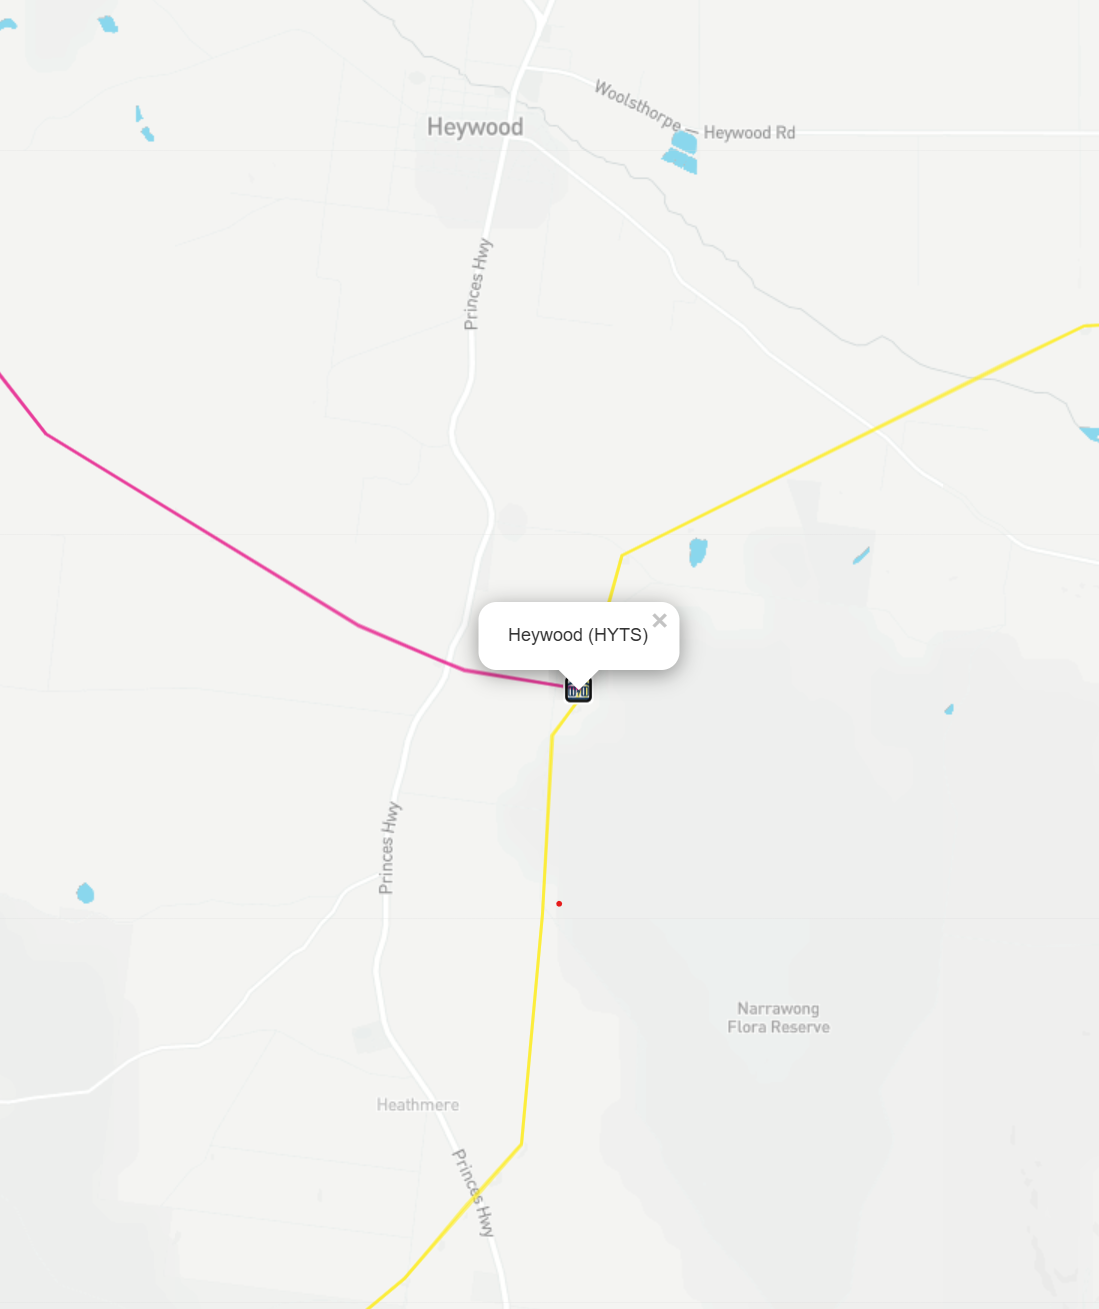
\includegraphics[width=0.7\textwidth]{\projectassetsdir/project-location.png} % Change example-image-a to the filename of your image
	\caption{Project location}
	\label{fig:project-location}
\end{figure}


	
	Project information is given as Table \ref{tab:projectinformation}.
	
% Project information	
{	
	\thicktablelines
	\begin{longtable}{|>{\columncolor{gray!20}}C{7cm}|C{8cm}|}
		\caption{Project Information}
		\label{tab:projectinformation} \\
		\toprule
		
		\rowcolor{tableheaderblue}
		\bfseries \color{white}Feature & \bfseries \color{white}Description \\
		\endhead
		\bottomrule \endfoot
		\csvreader[
		separator=semicolon,
		late after line=\\\hline,
		late after last line=,
		before reading={\catcode`\#=12},
		after reading={\catcode`\#=6}]%
		{report-assets/poc-data.csv}{1=\CSVItem,2=\CSVComment}{\CSVItem & \CSVComment}
	\end{longtable}
	
}
	
	
		\chapter{Reactive Capability}
	The reactive capability curves for \ac{Heywood BESS} at 35°C, 40°C and 50°C are shown in Figures \ref{fig:pq-curve-35degC}, \ref{fig:pq-curve-40degC} and \ref{fig:pq-curve-50degC}. The automatic access standard has been shown as a dotted line, and is defined by the upper corner points $P_{max}$=285 MW, $Q_{max}$=112.575 MVAr, $P_{max}$=285 MW, $Q_{min}$=-112.575 MVAr, and the lower corner points $P_{min}$=-285 MW, $Q_{min}$=-112.575 MVAr, $P_{min}$=-285 MW, $Q_{max}$=112.575 MVAr.
	
	
		\begin{figure}[H]
		\centering
		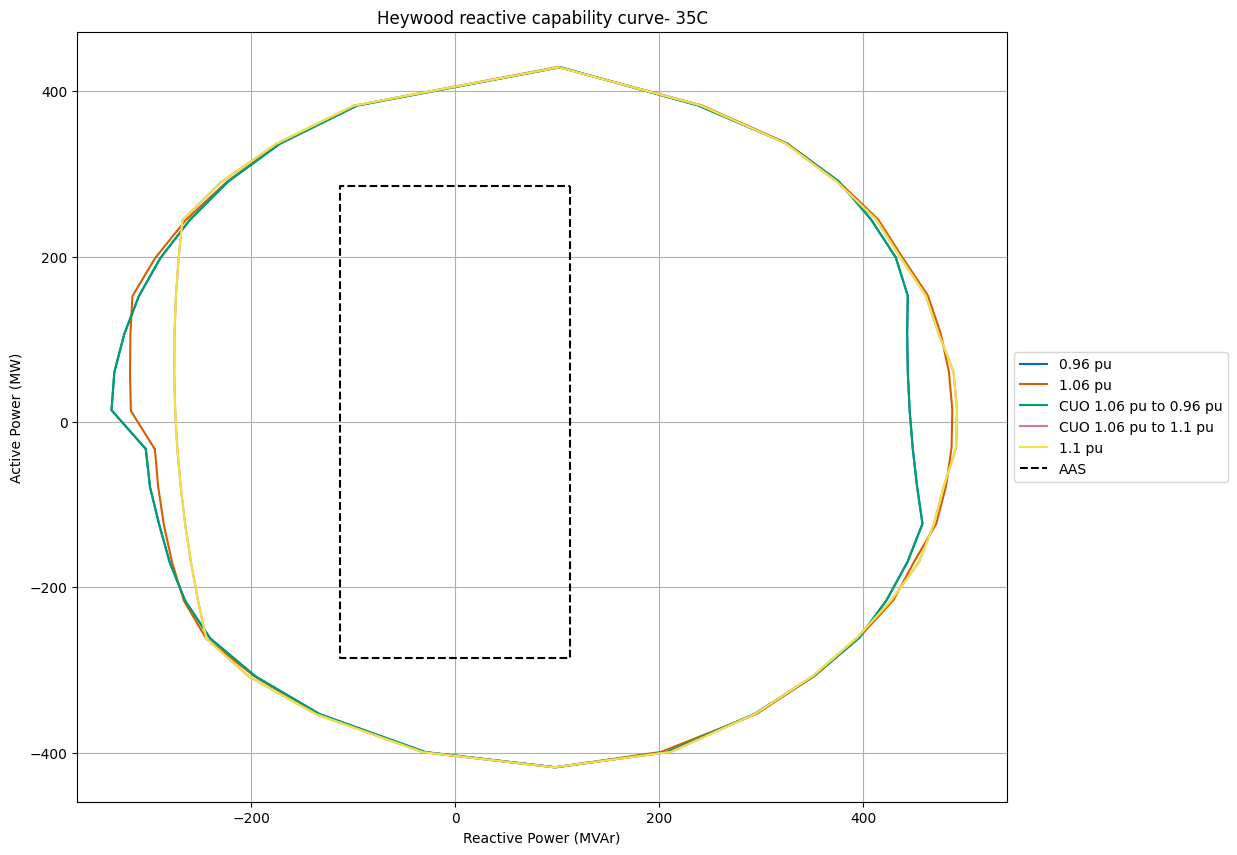
\includegraphics[width=0.8\textwidth]{\projectassetsdir/capability-curves/new_Heywood reactive capability curve- 35C.png}
		\caption{35°C Reactive capability curve for HEYWOODBESS}
		\label{fig:pq-curve-35degC}
	\end{figure}
	
	\begin{figure}[H]
		\centering
		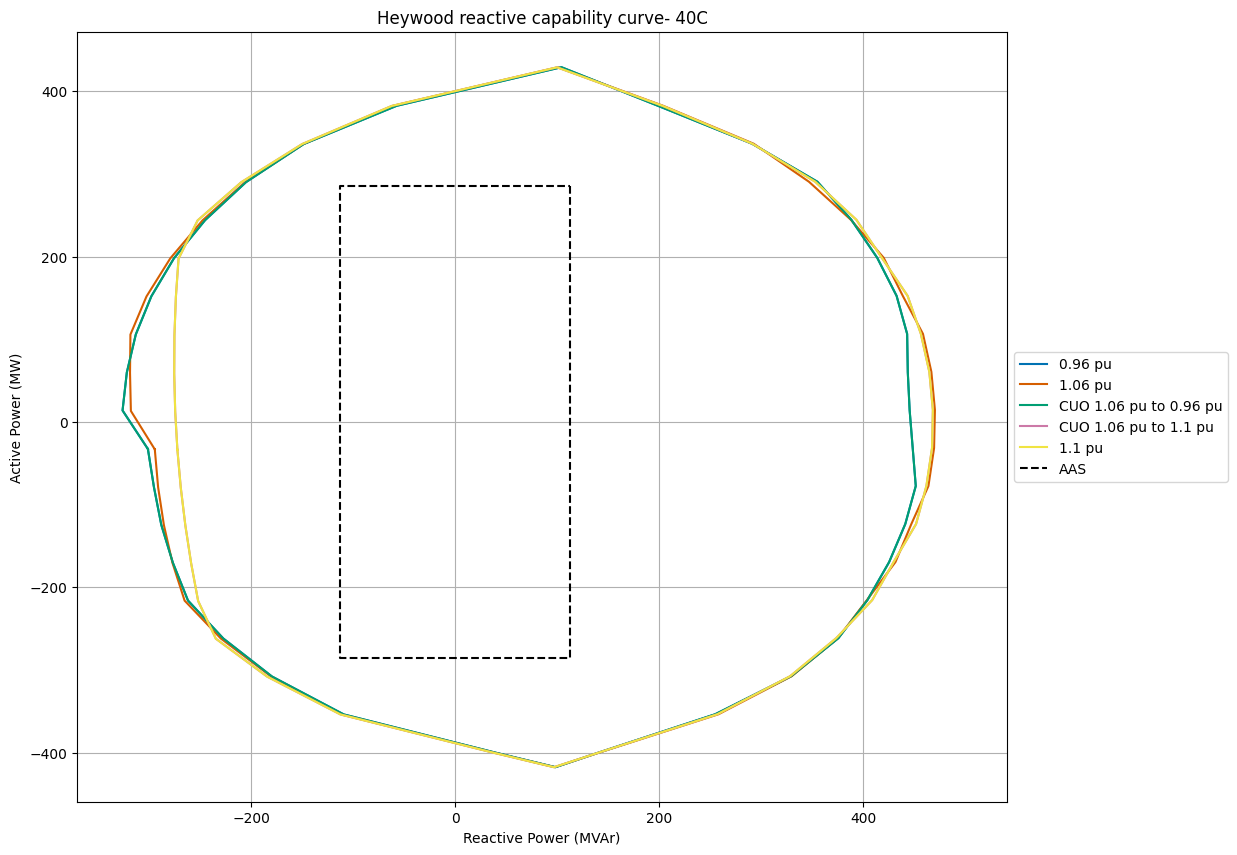
\includegraphics[width=0.8\textwidth]{\projectassetsdir/capability-curves/new_Heywood reactive capability curve- 40C.png}
		\caption{40°C Reactive capability curve for HEYWOODBESS}
		\label{fig:pq-curve-40degC}
	\end{figure}
	
	\begin{figure}[H]
		\centering
		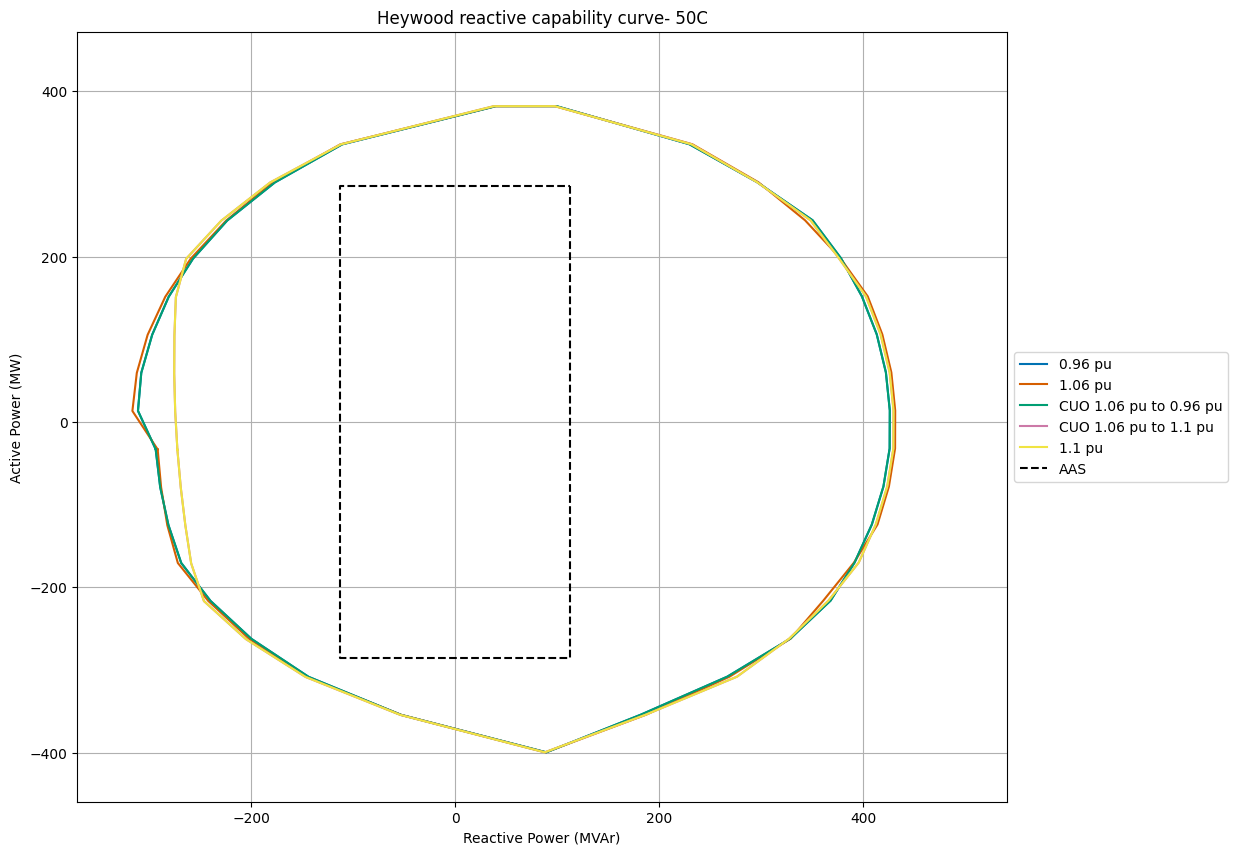
\includegraphics[width=0.8\textwidth]{\projectassetsdir/capability-curves/Heywood reactive capability curve- 50C.png}
		\caption{50°C Reactive capability curve for HEYWOODBESS}
		\label{fig:pq-curve-50degC}
	\end{figure}
	
	\chapter{Model Structure}
		
	\section{Layout}
	
	The HEYWOODBESS PSCAD model is divided into several regions:
	\begin{itemize}
		\item The main circuit diagram shows the \ac{SMIB} representation of the generating system.
		\item The \ac{PPC} region contains the Fluence Power Plant Controller and associated logic.
		\item The \ac{OLTC} region contains the tap changer logic for the grid transformer on load tap changers.
		\item The Grid Stimuli region defines the state of the circuit breakers in the SMIB model.
		\item The Plant Configuration section maps some key Global Substitution values, such as bases, to variables.
		\item The HMI control panel allows users to operate the model through manual configuration.
		\item The Plotting / Signal Derivation region at the bottom of the canvas is where signals, including derived signals, are assigned to output channels.
		\item The Automation region, which is used for automated execution, has been disabled by setting the global substitution variable AUTO_Automation_Mode_Enabled to 0.
		
	\end{itemize}
	
		
	\begin{figure}[H]
		\centering
		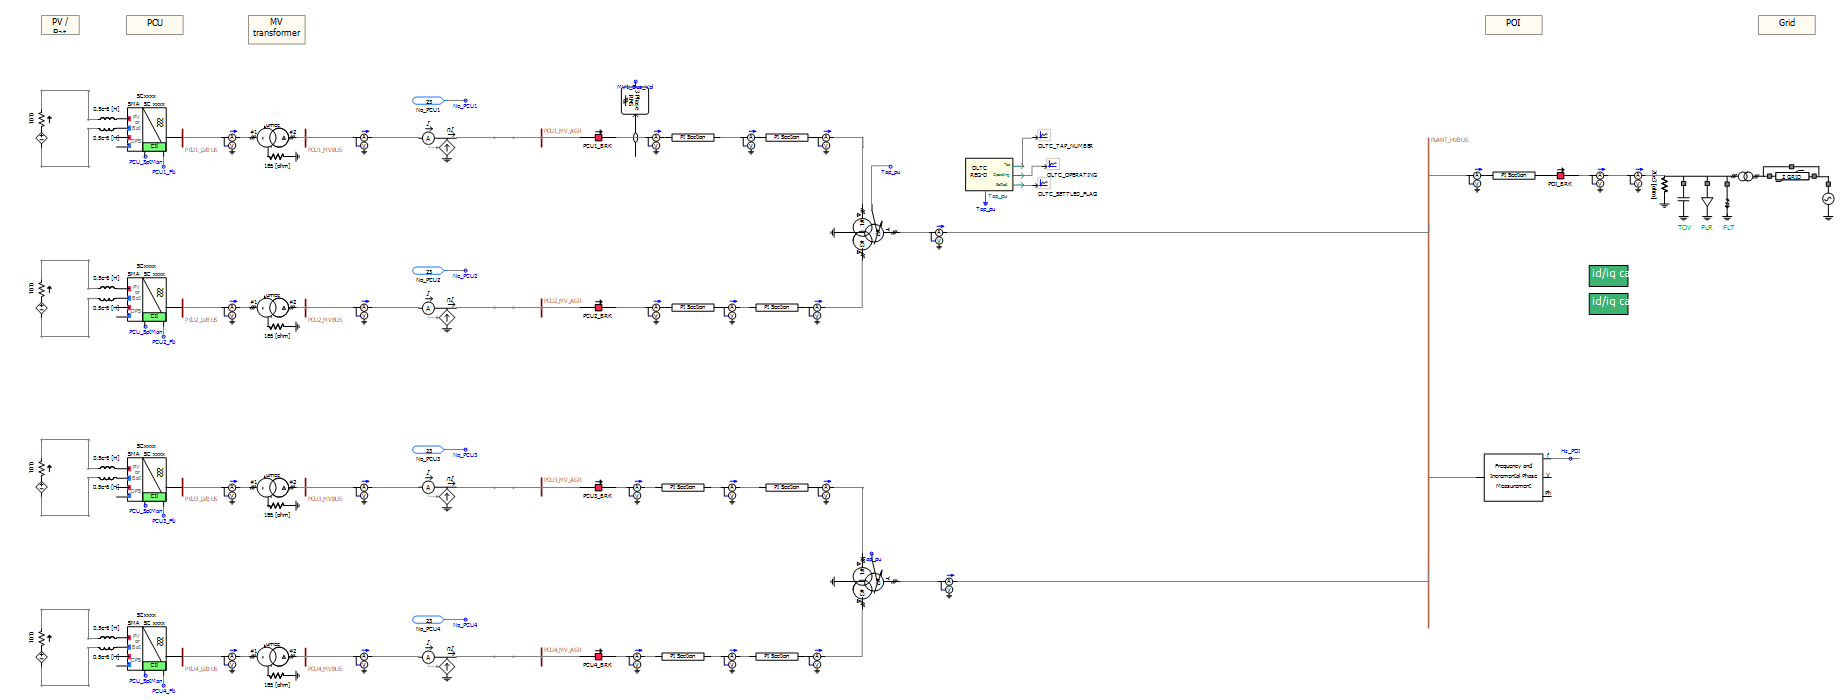
\includegraphics[width=0.9\textwidth]{report-assets/images/pscad-model-layout1.png}
		\caption{Model layout - main circuit}
		\label{fig:model-layout1}
	\end{figure}
	
	
		\begin{figure}[H]
		\centering
		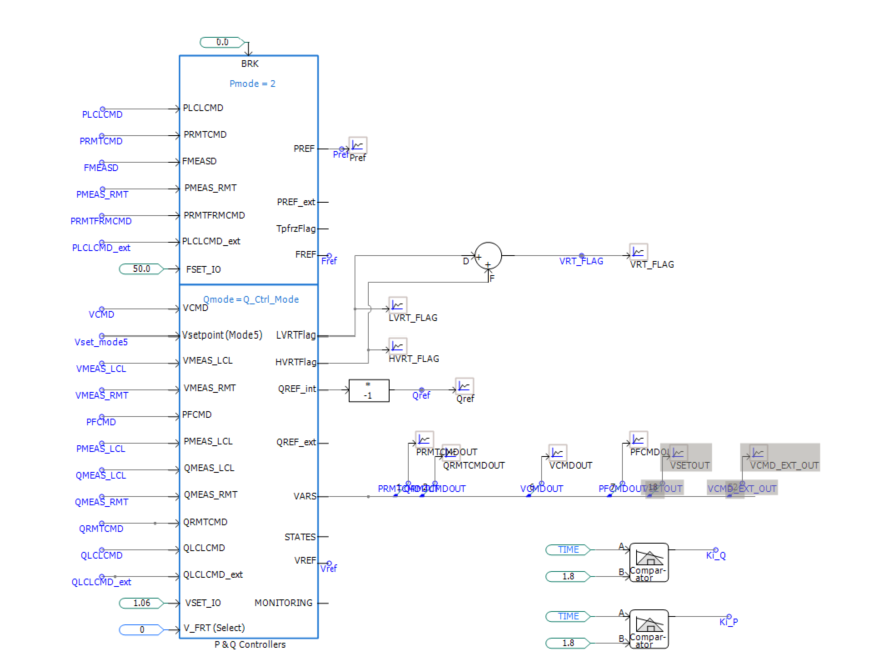
\includegraphics[width=0.9\textwidth]{report-assets/images/pscad-model-layout2.png}
		\caption{Model layout - P and Q control}
		\label{fig:model-layout2}
	\end{figure}
	
	
	\section{Dependencies}
	

	
	The HEYWOODBESS PSCAD model includes several libraries, which provide components for the main canvas:
	\begin{itemize}	
		\item SMA libraries SMA_Tools, FLNCPPC10_1, SC_Lib, SCAvg_Lib provide the converter transformer current scaling module, the PPC module, the converter module and an average voltage source converter module respectively (average voltage source converter module is not in use for this model).
		\begin{itemize}	
			\item SMASC_K_100015R03 is the active converter model version.
			\item FLNCPPC10_1 is the active PPC model version.
		\end{itemize} 
		\item Grid-Link module Pallet provides the grid model, the OLTC model, $i_d$ and $i_q$ calculation modules and control signal merging/unmerging blocks.
	\end{itemize} 
	All models are tested in PSCAD v5 and are provided with libraries for x86 and x86_64 architectures.
	
	
	\section{Parameter Configuration Files}
	
	The converter models read in text-based configuration files that contain the parameters that will remain fixed for the duration of the simulation (i.e. not set points). These are read by the model at the beginning of the simulation, then not read again during the run. The converter configuration file CfgFile57.txt has been supplied with the model.
	
	The PPC parameters are defined within the model itself; therefore separate parameter configuration file is required.
	

	
	
	\section{SMIB representation}

	Figure \ref{fig:model-screenshot1} shows the SMIB representation of the generating unit as presented in the PSCAD model. From right to left, the key elements are:
	\begin{itemize}
		\item The grid element, which provides facilities to configure the grid \ac{SCR} and X/R, apply faults and other disturbances.
		\item The point of connection.
		\item 1 x 275 kV underground cable between substation and point of connection (POC)		
		\item Two main three-winding 275/33/33 kV transformer with OLTC.
		\item Eight aggregated MV impedances representing the lumped impedance of 33kV feeders (modelled as X,R,B quantities).
		\item Four aggregated two-winding MV 33/0.69 kV converter transformers and current multiplier to represent all ninety-two (92) converters.
		\item Four lumped SCS 4600 UP-S converter model. 			
	\end{itemize}

	
		\begin{figure}[H]
		\centering
		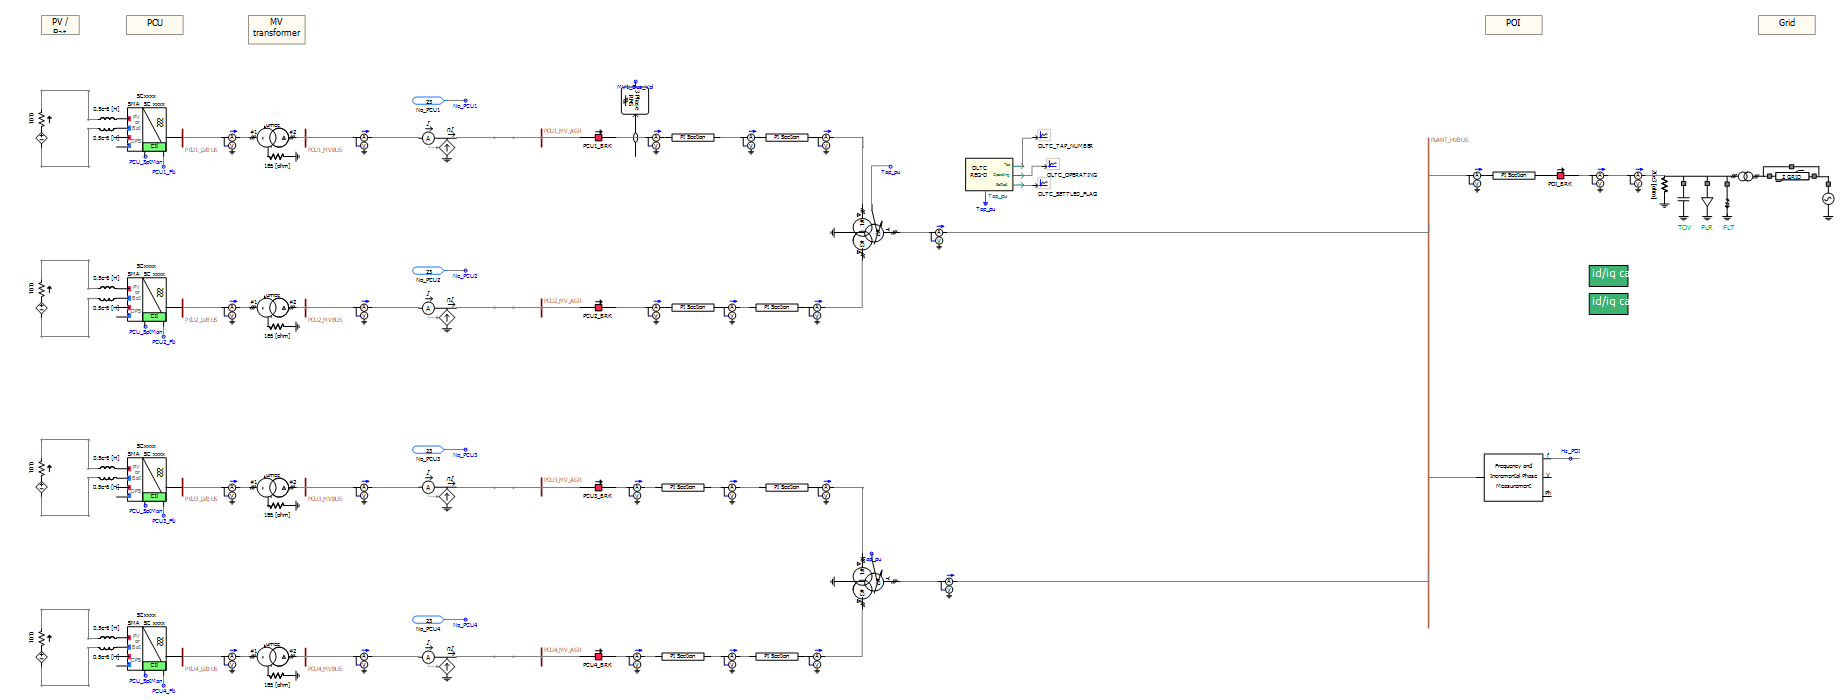
\includegraphics[width=\textwidth]{report-assets/images/pscad-model-layout1.png}
		\caption{SMIB representation of the generating system}
		\label{fig:model-screenshot1}
	\end{figure}
	
	Parameters for each electrical object and controller can be found in the appendix.

	\section{Control scheme configuration}
	

	 	This section will explain the default expected mode of operation for the plant, as well as how to operate the plant under alternative control modes if required, for both normal and abnormal operating conditions. 
	 	
	 	Under normal conditions, the plant will seek to control active and reactive power at its point of connection, via reference signals passed from the power plant controller to the converters. The normal operating voltage at the point of connection is 1.06 p.u. The plant also has a seperate operating mode for fault / overvoltage conditions, where the PPC may temporarily freeze to allow the converters to operate under reactive current control. Details of the operating modes and interactions between plant are explained in the following sections.
	 
	 	Fluence supplies the PPC FLNCPPC10_1 as an integrator, with parameters configurable directly within the model itself. SMA provides access to the majority of their converter settings through the configuration files CfgFile57.txt. 
	
	\subsection{Reactive Power Control Schemes}
		The FLUENCE PPC supports multiple reactive power control modes, selectable via the \textbf{General Reactive Power Parameters (Q) - Q Control Mode}. Under voltage disturbances, the plant operates under droop control and will diverge from its reference setpoint. The plant operates with a droop characteristic of 4.0\% on a 1 pu base, the voltage deadband is not used. The default reactive power control mode is the remote voltage control mode with voltage stack logic droop control (Q Control Mode=5). The available reactive power control modes and their configurations are summarised below:
		
		\subsubsection{Q Control Mode = Mode 5 — Remote Voltage Control Mode}
		
		When Q Control Mode is set to 5, the BESS enters remote voltage control mode, which operates with \ac{VSL} droop logic. In order to use this control mode the VSL is required to be always enabled (General Reactive Power Parameters(Q) - Voltage stack Logic). Key parameters to adjust reactive power control are shown below:
		
		\begin{itemize}
			\item Q Control Mode - must be set to Mode 5 for the PPC to operate in remote voltage control mode.
			\item General Reactive Power Parameters(Q) - Voltage Stack Logic - must be set to Enable when operating in Mode 5.
			\item VCMD - can be adjusted to set the remote voltage setpoint.
		\end{itemize}
		
		\subsubsection{Voltage Droop Characteristics}
		
		
		Given the 4\% voltage droop characteristic of the Heywood BESS, the corresponding relationship is defined as follows:
		
		
		\[
		\text{Droop} =  \left[ \frac{\text{p.u.}}{\text{p.u.}} \right] = \frac{(U - U_{\text{set}})/U_n}{(Q - Q_{\text{set}})/Q_n} = \frac{U - U_{\text{set}}}{Q - Q_{\text{set}}} \cdot \frac{Q_n}{U_n}
		\]
		(with Qn = 112.575 MVAr)
		
		
		
		\begin{figure}[H]
			\centering
			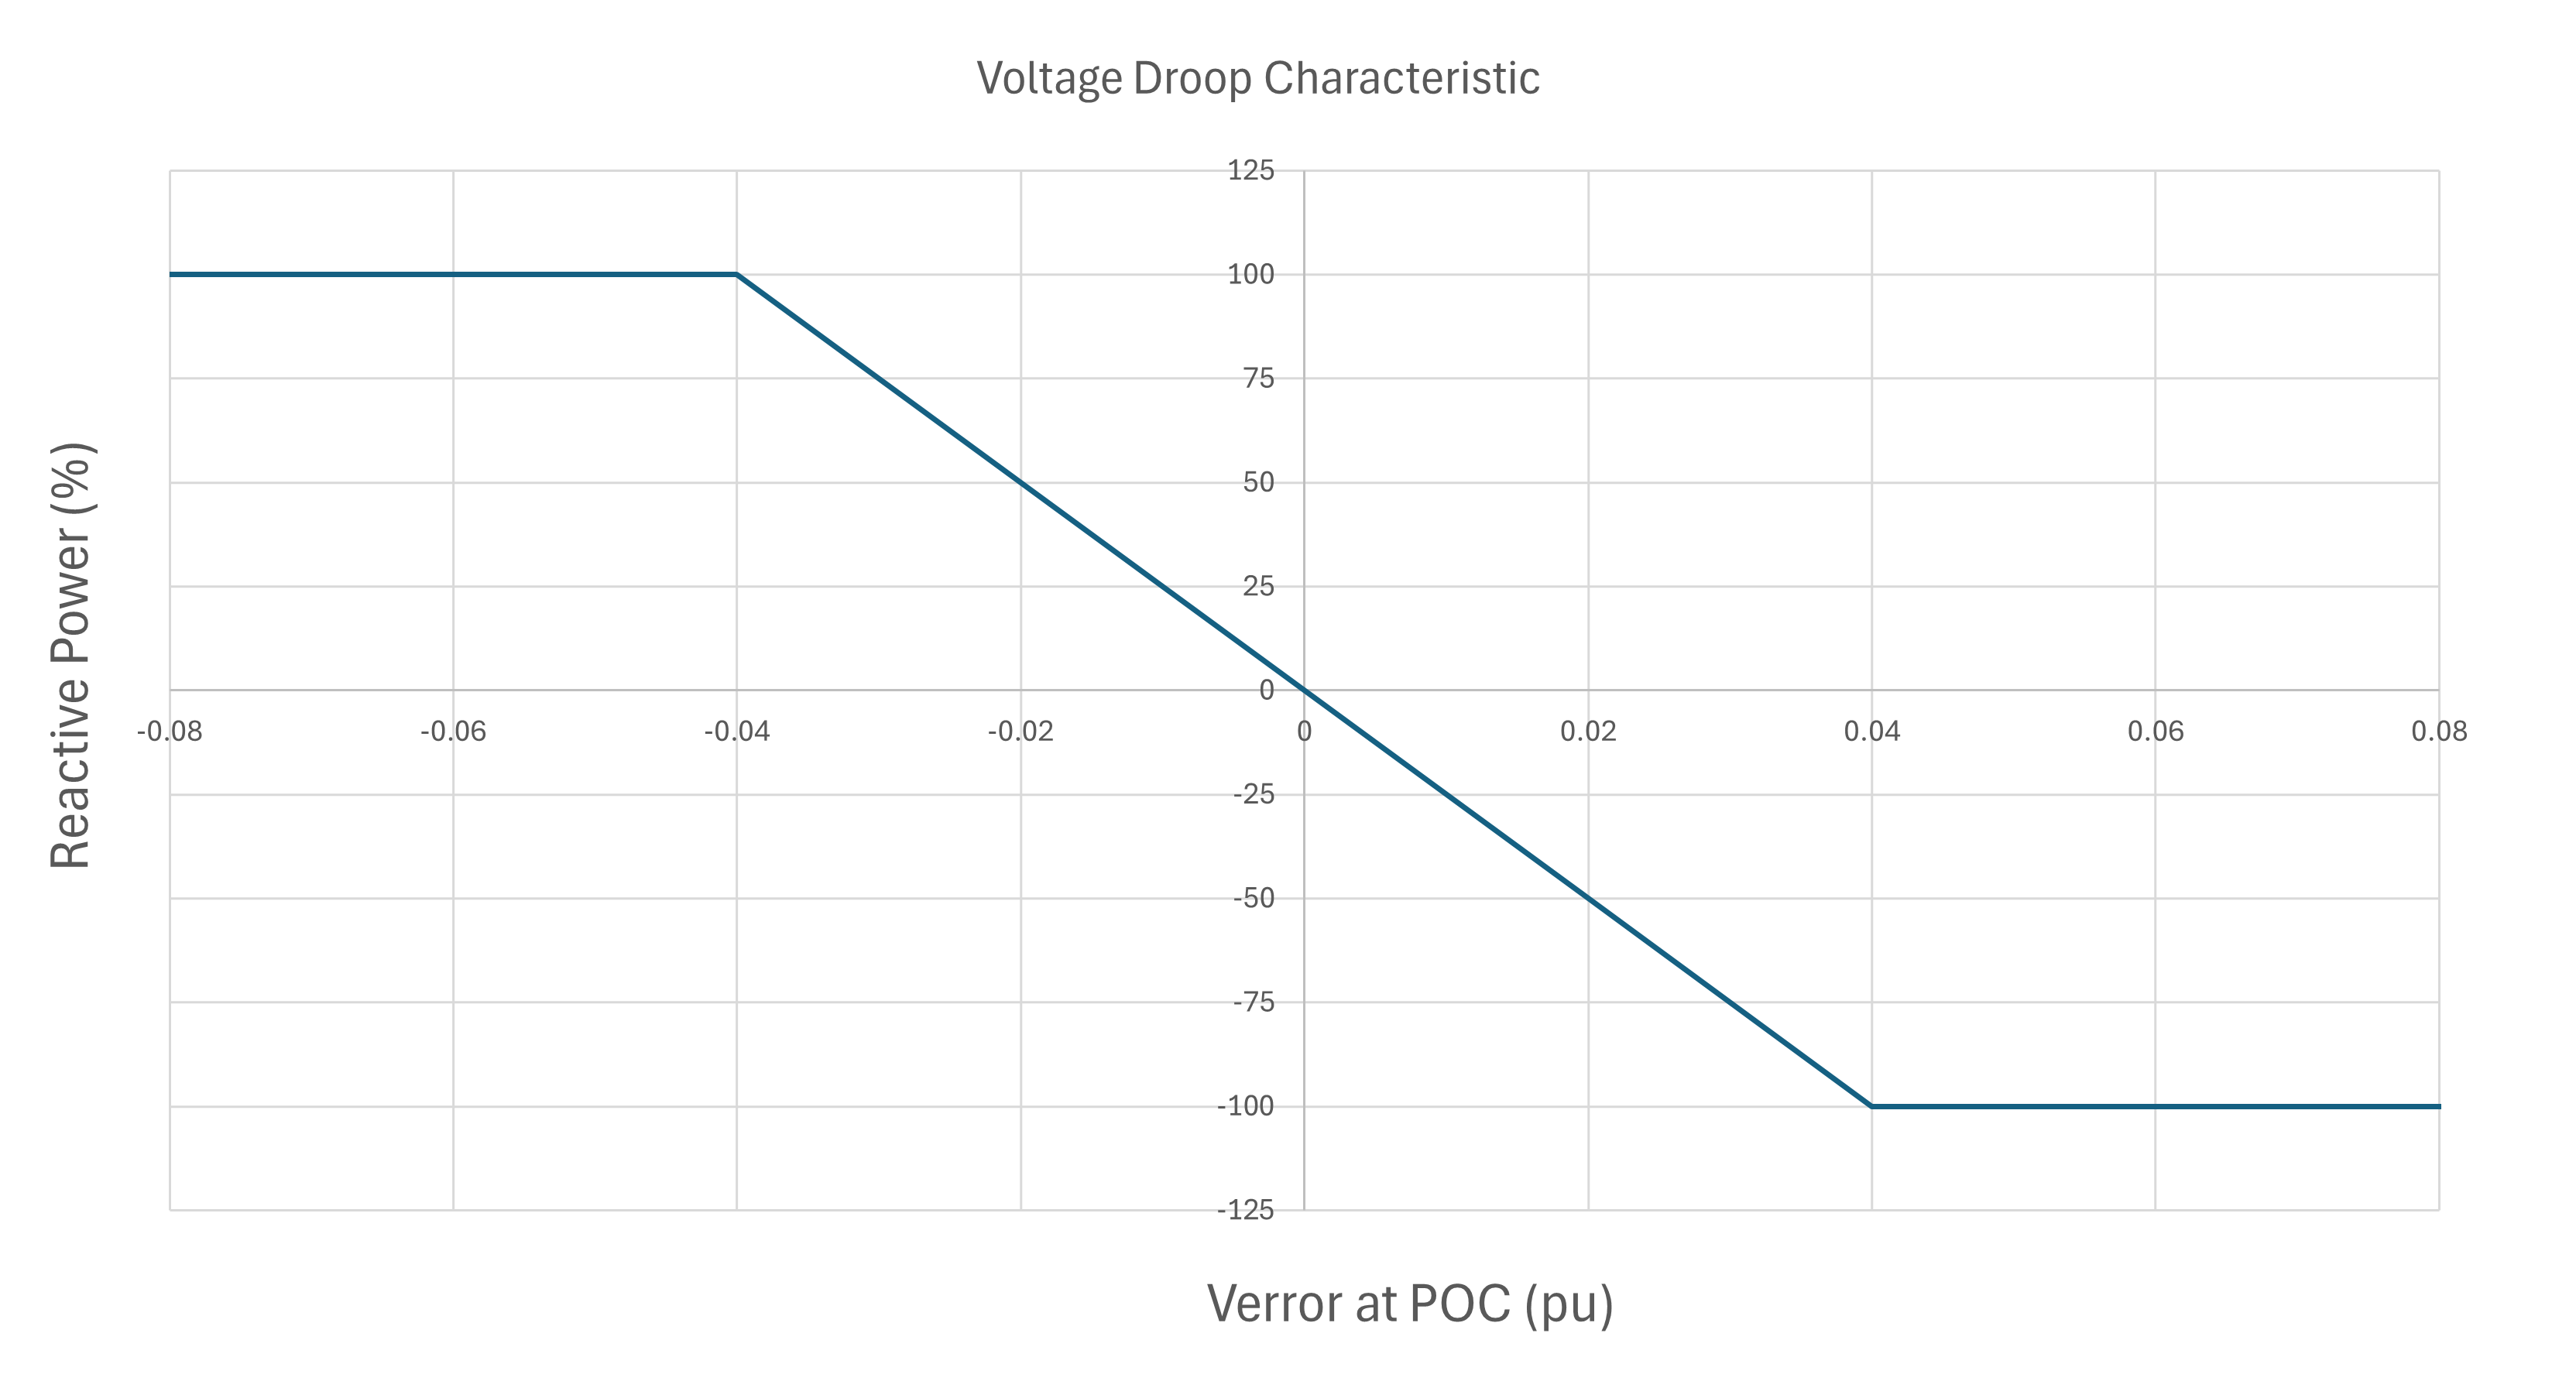
\includegraphics[width=0.9\textwidth]{report-assets/images/vdroop-char.png}
			\caption{Voltage droop characteristic}
			\label{fig:vdroop-char}
		\end{figure}
		
		\dansquicktable{|C{4cm}|C{4cm}|C{4cm}|C{4cm}|}
		{Voltage droop characteristic tabulated}
		{v-droop-char}
		{\bfseries \color{white} & \bfseries \color{white}Normal voltage (pu) & \bfseries \color{white}Voltage at POC (pu)) & \bfseries \color{white}Reactive Power (MVAr)}
		{report-assets/v-droop-char-new.csv}
		
		
		\subsubsection{Q Control Mode = Mode 2 — Power Factor Control Mode}
		
		When Q Control Mode is set to 2, the BESS operates in power factor control mode, controlling power factor at its point of connection. Key parameters to adjust power factor control are shown below. Note that voltage stack logic should be disabled when operating in Mode 2.
		
		\begin{itemize}
			\item Q Control Mode - must be set to Mode 2 for the PPC to operate in power factor control mode.
			\item PFCMD - can be adjusted to set power factor target at the POC.
		\end{itemize} 
		
		\subsubsection{Q Control Mode = Mode 3 — Remote Reactive Power Control Mode}
		
		When Q Control Mode is set to 3, the BESS enters remote reactive power control mode. In this mode, the reactive power at the point of connection is regulated based on a command signal QRMTCMD. Key parameters to adjust droop control are shown below. Note that voltage stack logic should be disabled when operating in Mode 3.
		
		\begin{itemize}
			\item Q Control Mode - must be set to Mode 3 for the PPC to operate in remote reactive power control mode.
			\item QRMTCMD - can be adjusted to control the reactive power at the remote branch.
		\end{itemize}
		
		\subsubsection{OLTC control}

		The 275/33/33 kV three-winding grid transformers are equipped with an on-load tap changer. The \ac{OLTC} have been specified to regulate the voltage at the medium voltage side of the main transformers to be 1 p.u.The OLTC auto-voltage regulation (AVR) relay utilises a deadband ensuring that the voltage target is achieved to within $\pm$ 0.015 pu. An initial tap change in response to a voltage deviation beyond the control dead band is undertaken after a defined delay of 20 seconds. This is commonly understood as an AVR constant time program. 
		
		The transformer is set to operate with a time delay of 20 seconds and 7s mechanical operation time. If after a single tap change operation the voltage is still outside the deadband, another tap will be expected after an additional 20 seconds. This time delay has been selected to ensure no unwanted interference between primary and secondary control loops while ensuring it is fast enough to ensure the generator maintains continuous uninterrupted operation for a variety of network disturbances.
		
		{
			\thicktablelines
			\begin{longtable}{|C{6cm}|C{4cm}|} 
				\caption{Grid transformer OLTC Details}
				\label{tab:main-transformer}
				\\	
				\toprule
				
				\rowcolor{tableheaderblue}
				\bfseries \color{white}Parameter & \bfseries \color{white}Value\\
				\endhead
				\bottomrule \endfoot
				\csvreader[
				separator=semicolon,
				late after line=\\\hline,
				late after last line=,
				before reading={\catcode`\#=12},
				after reading={\catcode`\#=6}]%
				{report-assets/main_transformer.csv}{1=\CSVParameter,2=\CSVValue}{\CSVParameter &\CSVValue}
				\\\hline
			\end{longtable}
		}
		
		
		\subsection{Active power and frequency control}
		
		The \ac{PPC} regulates active power output through setpoint commands to the converters to target a fixed active power setpoint at the point of connection. Under frequency disturbances, the plant operates under droop control and will diverge from its reference setpoint. The plant operates with a droop characteristic of 5.0\% on a 50 Hz base, and a frequency deadband of +/- 0.015 Hz. 
		
		The PPC can operate in both local active power control and remote active power control, to be defined by the user. The PPC operates in remote active power control mode by default. This characteristic is shown in Figure \ref{fig:fdroop-char} and Table \ref{tab:frq-droop-char-new}. 
		\subsubsection{P Control Mode = Mode 1 — Local Active power Control Mode}
		
		Key parameters for local active power and frequency control are shown below: 
		
		\begin{itemize}
			\item P Control Mode - must be set to mode 1 to enable local active power control mode
			\item PLCLCMD - can be adjusted to set local active power
		\end{itemize}
		
		\subsubsection{P Control Mode = Mode 2 — Remote Active power Control Mode}
		
		Key parameters for remote active power and frequency control are shown below: 
		
		\begin{itemize}
			\item P Control Mode - must be set to mode 2 to enable remote active power control mode
			\item PRMTCMD - can be adjusted to set the remote active power command
		\end{itemize}
		
		\subsubsection{Frequency Droop Characteristics}
		Given the 5\% frequency droop characteristic of the Heywood BESS, the corresponding relationship is defined as follows:
		
		
		\[
		\text{Droop=} \left[ \frac{\text{MW}}{\text{Hz}} \right] = \frac{1}{\Delta f / \Delta P} = \frac{\Delta P}{\Delta f} = \frac{P - P_{\text{set}}}{f - f_{\text{set}}}
		\]
		
		
		\begin{figure}[H]
			\centering
			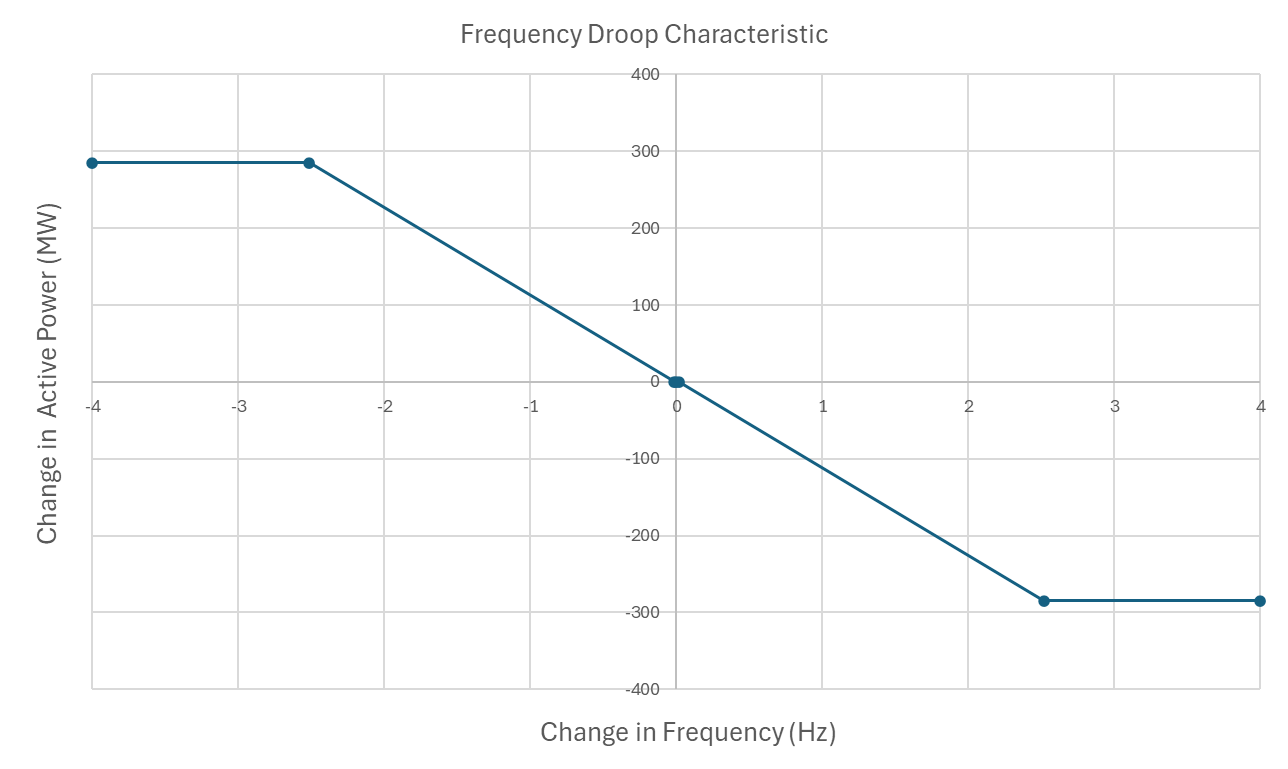
\includegraphics[width=0.9\textwidth]{report-assets/images/fdroop-char.png}
			\caption{Frequency droop characteristic}
			\label{fig:fdroop-char}
		\end{figure}
		
		
		{	
			\thicktablelines
			\begin{longtable}{|C{4cm}|C{4cm}|}%eg: {|C{5cm}|C{5cm}|}
				\caption{Frequency droop characteristic tabulated}%eg: {FRT parameters}
				\label{tab:frq-droop-char-new} \\% eg: {tab:frt-parameters} \\
				\toprule
				\rowcolor{tableheaderblue}
				\bfseries \color{white}Change in Frequency (Hz) & \bfseries \color{white}Active Power (MW) \\%eg: {\bfseries \color{white}Parameter & \bfseries \color{white}Unit & \bfseries \color{white}Value} \\
				\endhead
				\bottomrule \endfoot
				\csvreader[
				late after line=\\\hline,
				late after last line=,
				before reading={\catcode`\#=12},
				after reading={\catcode`\#=6}]% 
				{report-assets/frq-droop-char-new.csv}{}{\csvlinetotablerow} 
				\\\hline
			\end{longtable}
		}	
		
		\subsection{Fault ride through mode}
		
		Unlike a typical grid following plant, the grid forming BESS converters do not have a defined set of voltages at which they enter an FRT mode. The converters instead have a "virtual impedance" mode, which is activated following large voltage step change deviations at the converter terminals, which serves as its FRT mode. Under this mode, the plant injects current according to the reciprocal of a defined impedance, which acts as an equivalent to a "k-factor" commonly used in grid following FRT applications.
		
		Seperately to the converters, the plant PPC will freeze following point of connection voltages dropping below 0.85 or above 1.15 p.u. The risk of PPC windup during FRT causing disturbances in operation is therefore mitigated.
		
		\section{Protection}
		
		The converters are equipped with frequency and voltage protection, which are set to keep the plant connected as per the NER requirements, but trip to avoid the plant supplying onto a faulted system. The frequency protection characteristic is shown in Figure \ref{fig:fprotection}. The voltage protection characteristic is shown in Figure \ref{fig:vprotection}.
		
		\begin{figure}[H]
			\centering
			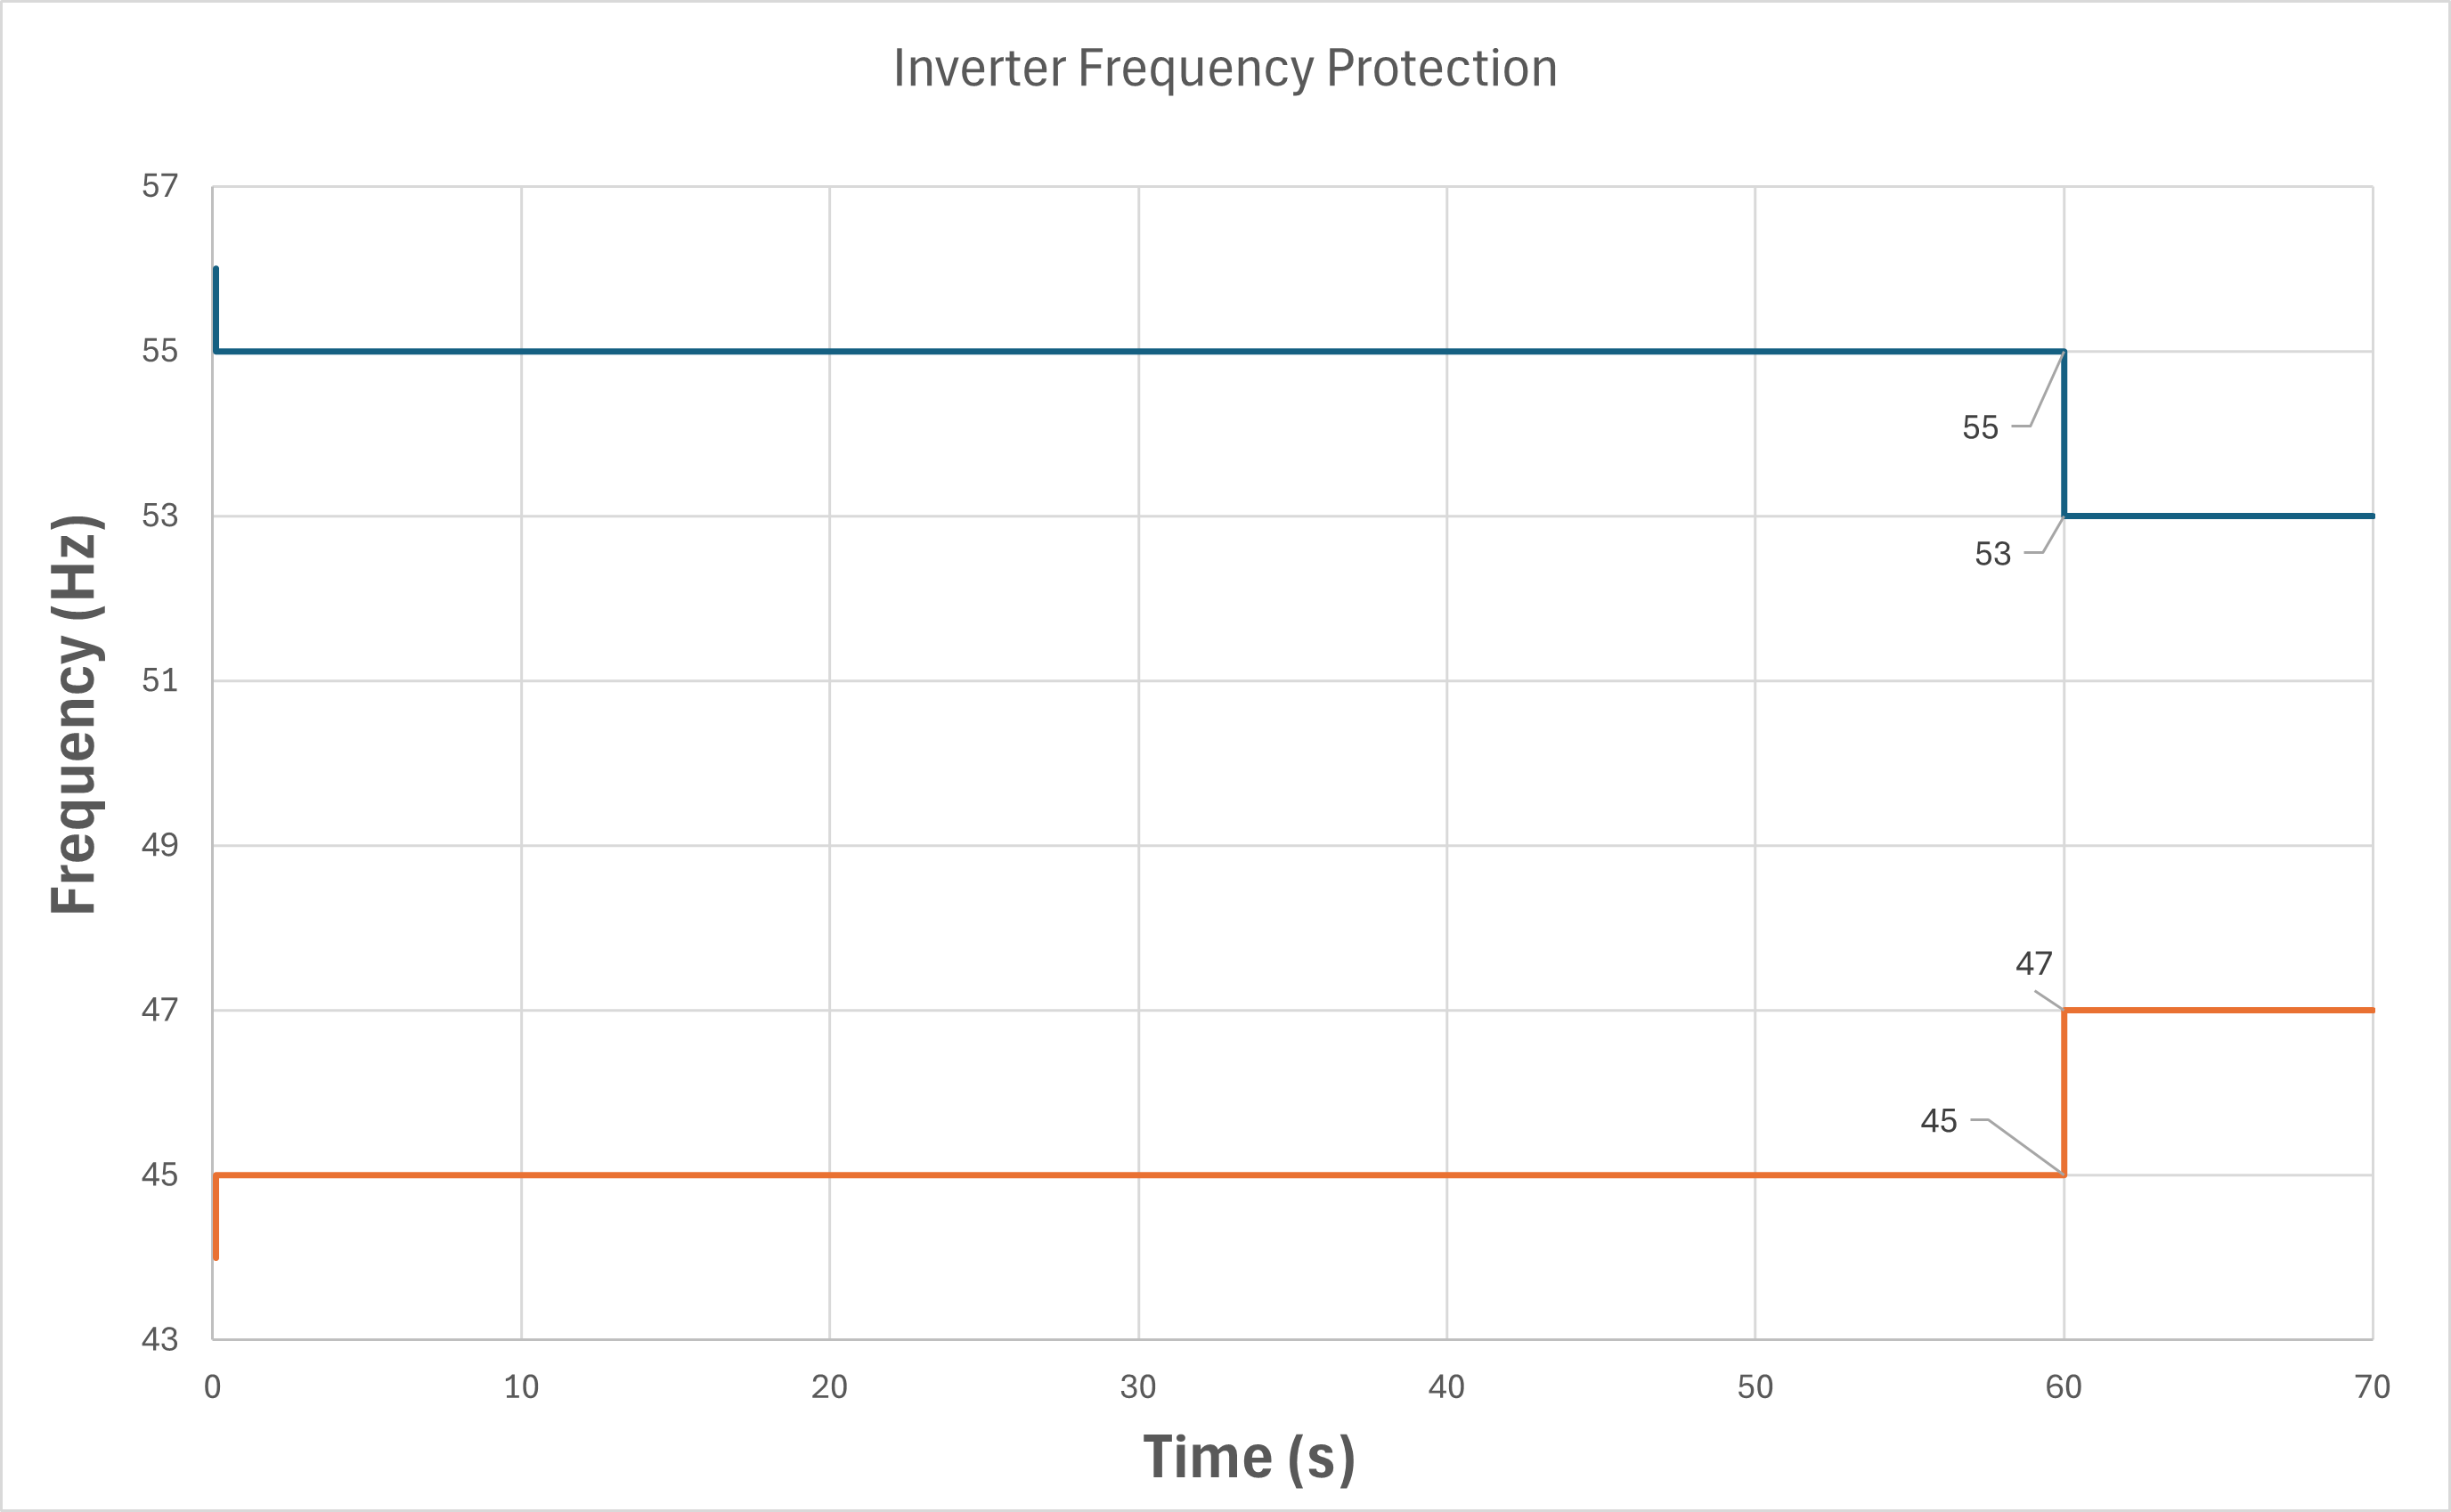
\includegraphics[width=0.6\textwidth]{report-assets/images/fprotection.png}
			\caption{Frequency protection characteristics}
			\label{fig:fprotection}
		\end{figure}
		
		\begin{figure}[H]
			\centering
			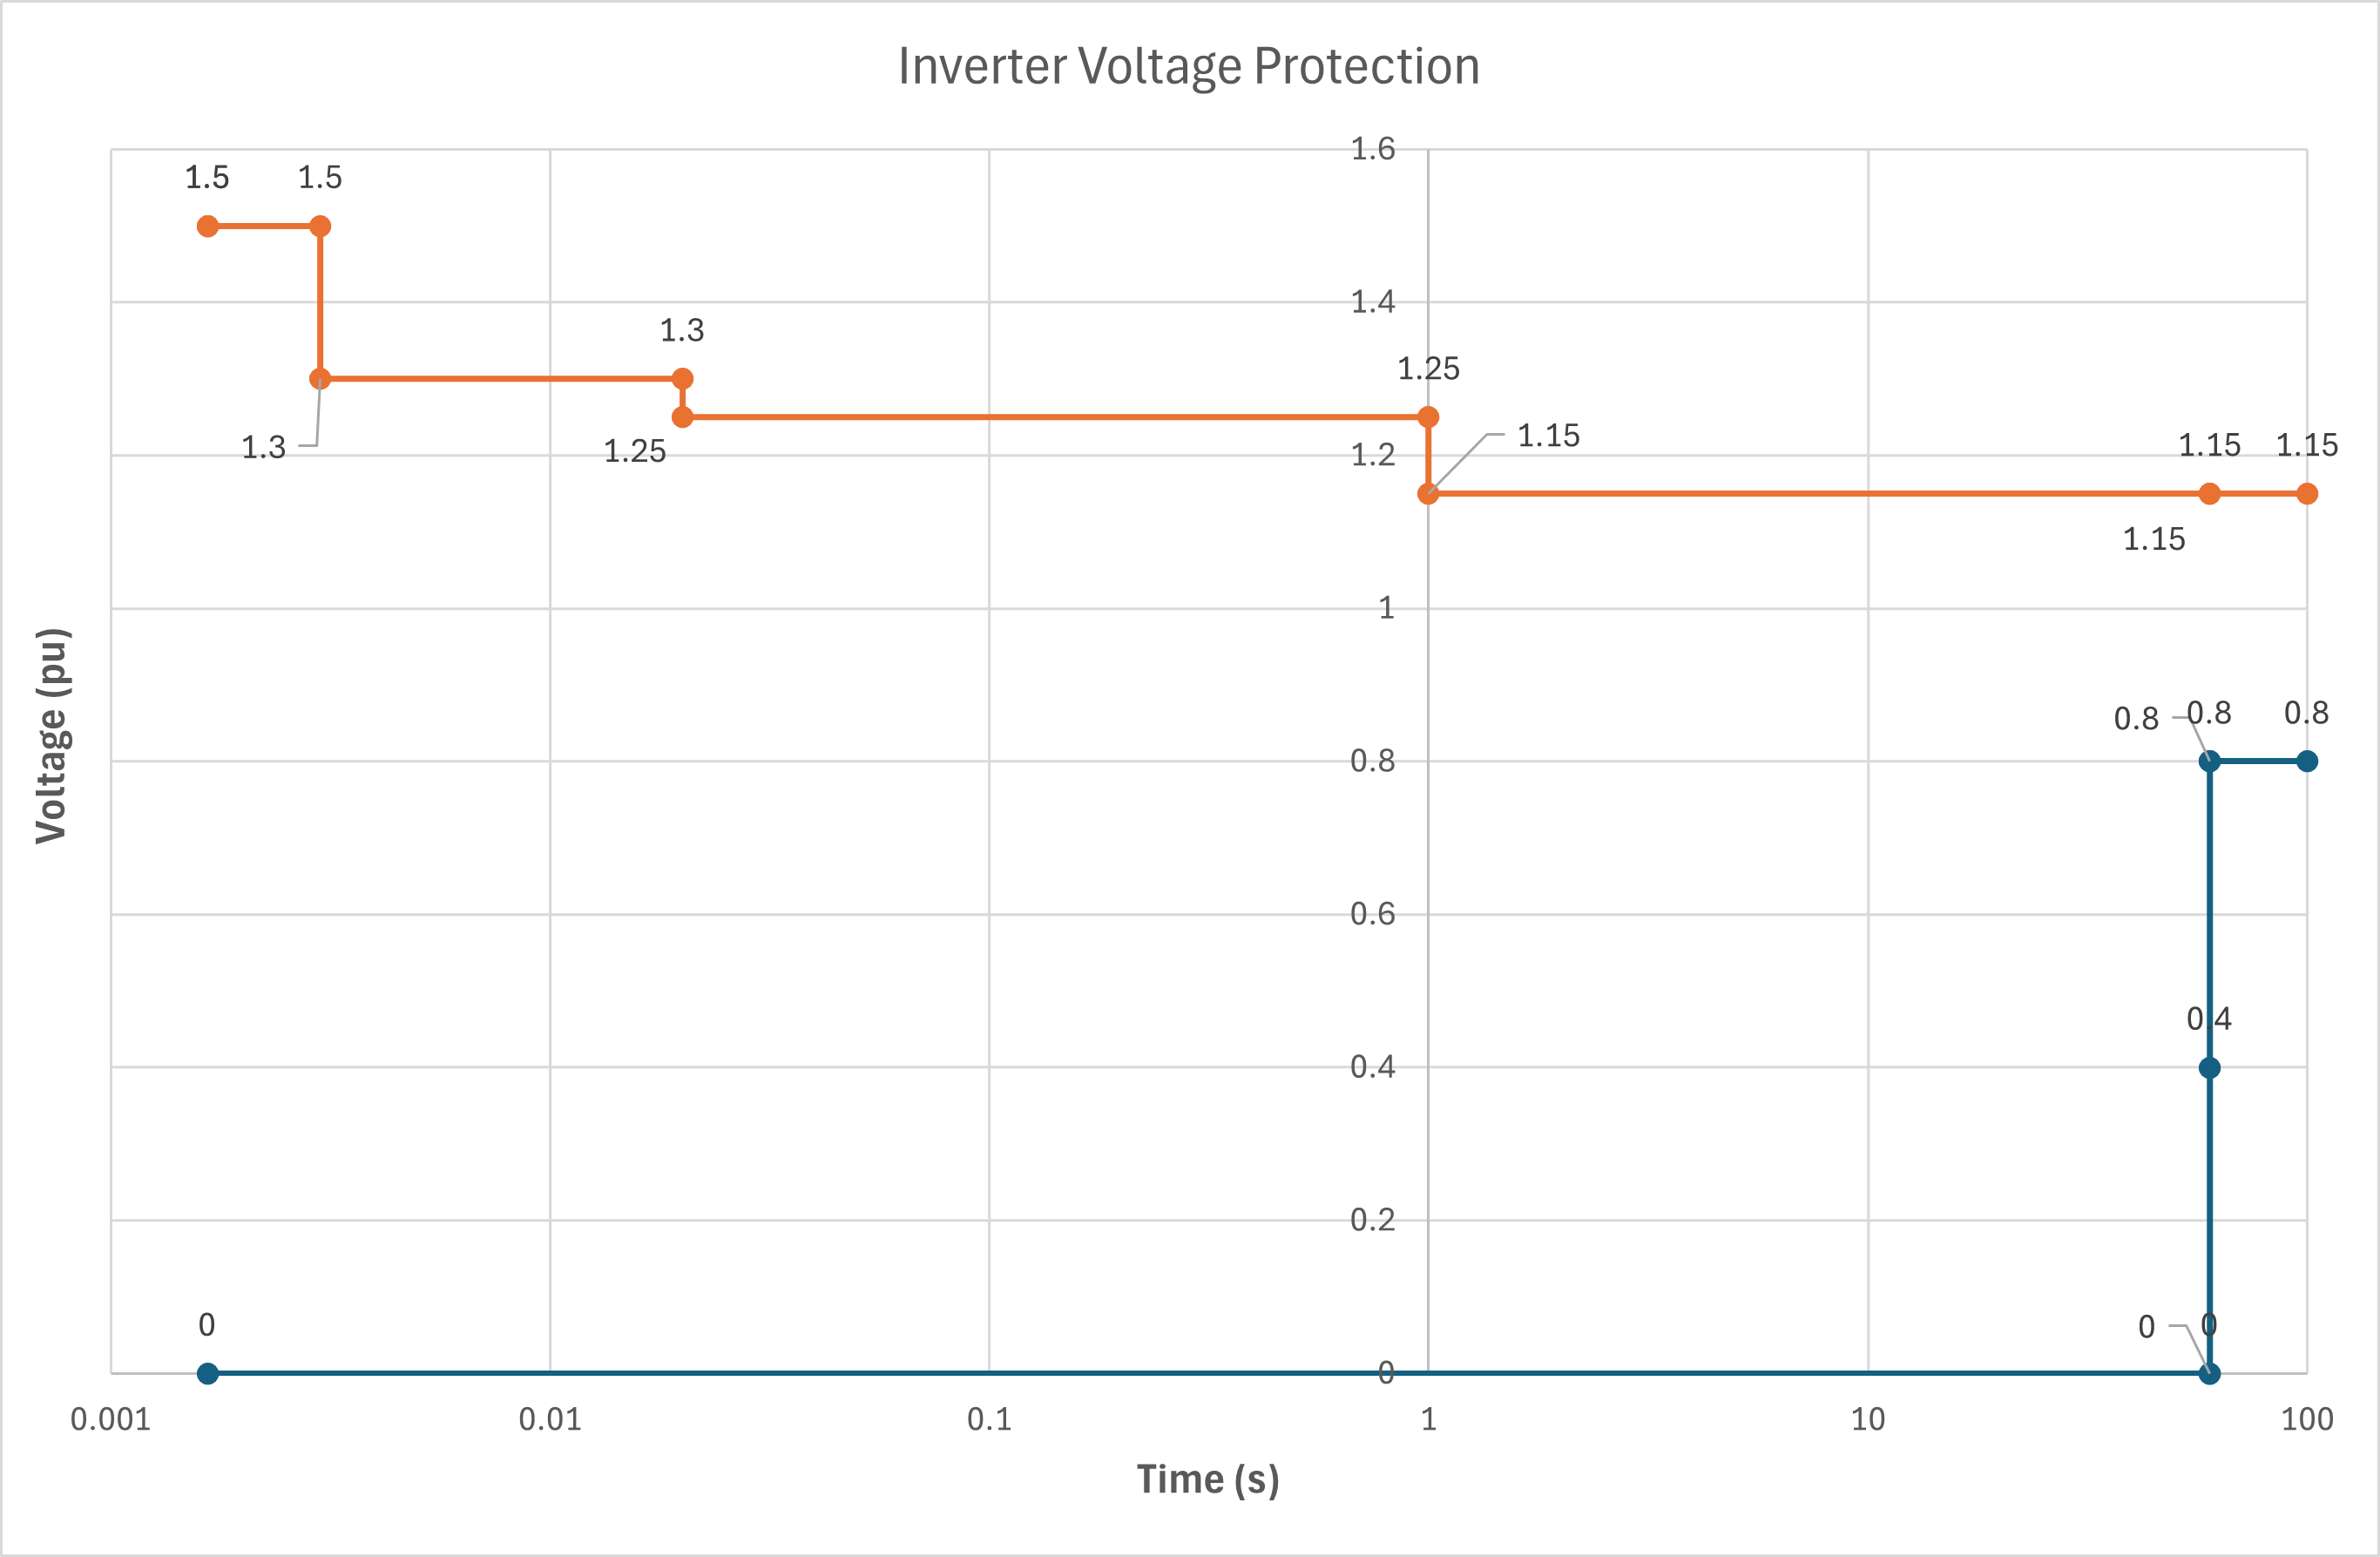
\includegraphics[width=0.6\textwidth]{report-assets/images/vprotection-new.png}
			\caption{Voltage protection characteristics}
			\label{fig:vprotection}
		\end{figure}
		
		\section{Simulation with a reduced number of converters}
		
		To perform simulations with a reduced number of converters on each branch,$n$, the following parameters need to be adjusted in the model
		
		\begin{itemize}
			\item Modify the No\_PCU signal above each branch to adjust the number of converters to the correct amount.
			\item Modify the MVA rating of the "BESS MVA" variable in the PPC.
			
		\end{itemize}
		
		All other parameters are in pu and will be adjusted automatically.
	
	\subsection{Initialisation-specific modifications}
	
	The model initialises in 7 seconds at all combinations of Pmax/Pmin, Qmax/Qmin and SCRmin/SCRmax. Note: The converter control mode is initially set to 21521 for the first 6 seconds to enable fast initialization, and then it switches back to 22321 after 6 seconds.
	
	
	\subsection{HMI controls}
	
	When automation mode is disabled, control of set points and disturbances is available from the control panels in the $PPC$ region of the canvas, as shown in Figure \ref{fig:control-canvas}. The controls in this category can be grouped as follows:
	\underline{Grid representation configuration section:}
	\begin{itemize}	
		\item Grid state determines whether to use the ‘initial’ fault level and X/R provided or the ‘recovery’ fault level and X/R. Most studies will be performed with a single fault level and X/R, so this should be set to ‘INIT,’ but studies involving a switch to a different SCR mid simulation can do so by toggling the Grid state to ‘RECOV.’
		\begin{itemize}	
			\item Init Grid MVA and Init Grid X/R are the initial fault level and X/R values for the grid.
			\item Rec. Grid MVA And Rec. Grid X/R are the ‘recovery’ fault level and X/R values to be switched to.\\ \bfseries{IMPORTANT: these must be set to values greater than 0 even when not used, or PSCAD may treat the impedance as a short circuit. It is suggested to use values equivalent to SCR=1 when not in use.}
		\end{itemize} 
		\item Infinite Grid: ‘INF’ short circuits the grid impedance, directly connecting the slack bus to the Connection Point. ‘GRID’ puts the grid impedance in between these buses.	
		\item Vslack (pu) sets the voltage of the slack bus.
		\item Fslack (Hz) sets the frequency of the slack bus.
		\item Grid phase (deg) sets the phase angle of the slack bus (default = 0°)
		\item Vpoc disturbance (pu) uses a dummy transformer at the Connection Point to apply a percentage voltage change at the Connection Point.
	\end{itemize}
		\underline{TOV (Temporary Over-Voltage) section:}
	\begin{itemize}
		\item Fault Duration Sec sets the number of seconds that the next TOV will be applied for.
		\item Shunt uF sets the size of the shunt to be applied.
		\item TOV Fault Trigger initiates the application of the TOV capacitor for the required duration. It is automatically reset after this.
	\end{itemize}
	\underline{Faults section:}
	\begin{itemize}
		\item Fault X/R sets the X/R of the fault impedance.
		\item Fault Type sets the faulted phases based on the PSCAD fault enumeration (e.g. 7 is a balanced fault).
		\item Fault duration pre-defines the duration of the fault in seconds.
		\item Fault Strategy allows the user to configure the fault based on a per unit residual voltage (‘Ures’) or a ratio of fault impedance to source impedance (Zf/Zs).
		\begin{itemize}
			\item If Ures is selected, only the Residual Voltage (pu) slider is used.
			\item If Zf/Zs is selected, the ratio of Zf/Zs is set using the Zf/Zs slider, then an additional R and X can be added to the calculated fault impedance. This allows, for example, a 10Ω fault could be applied with Zf/Zs = 0, Rf Offset = 10, Xf Offset = 0. 
		\end{itemize}
		\item Fault trigger engages a fault for the duration specified in Fault Duration
	\end{itemize}
	
	\begin{figure}[H]
		\centering
		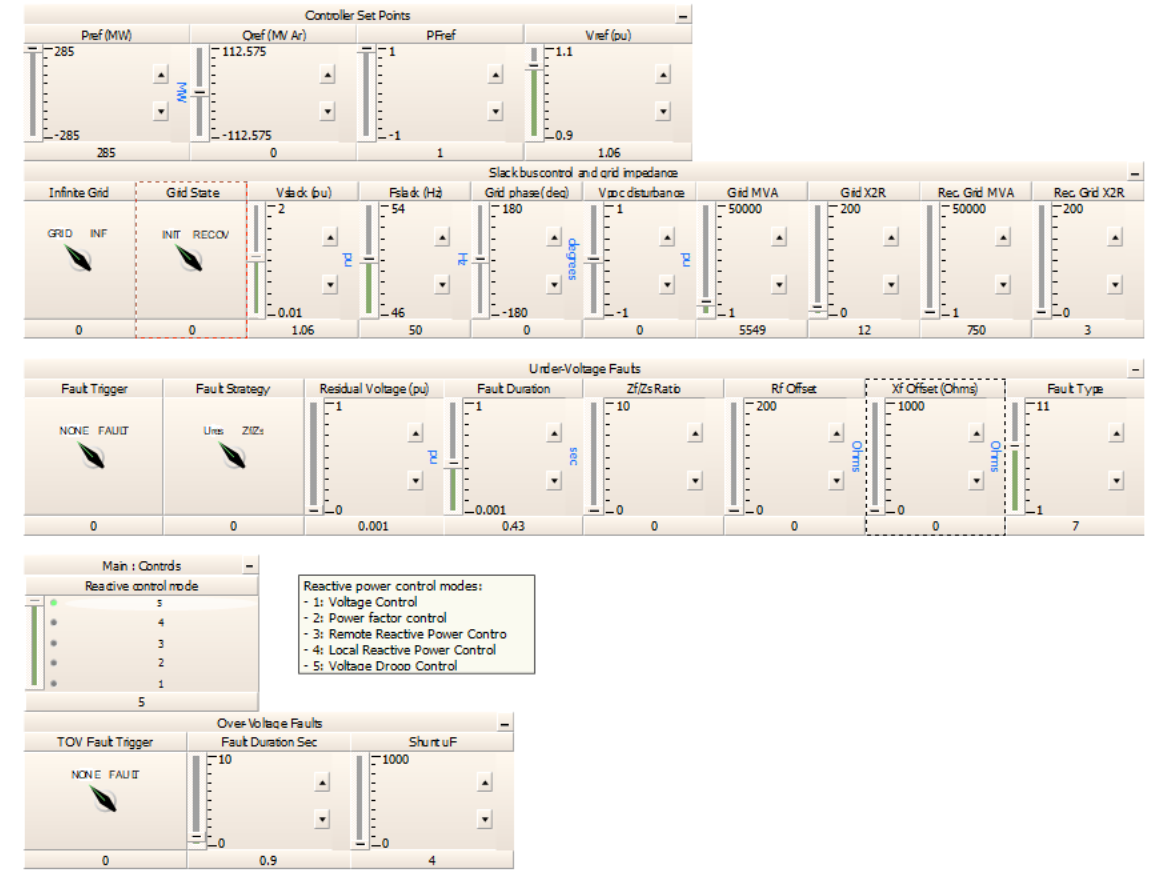
\includegraphics[width=\textwidth]{report-assets/images/PPC-CANVAS.png}
		\caption{Controls region of the canvas}
		\label{fig:control-canvas}
	\end{figure}
	

	

	These set points are fed into the PPM module in the model as shown in Figure \ref{fig:ppm-inputs}.  PPC input/output table in Fluence PPC manual as shown in Table \ref{tab:ppc-inputs-table}.
	
	
	\begin{figure}[H]
		\centering
		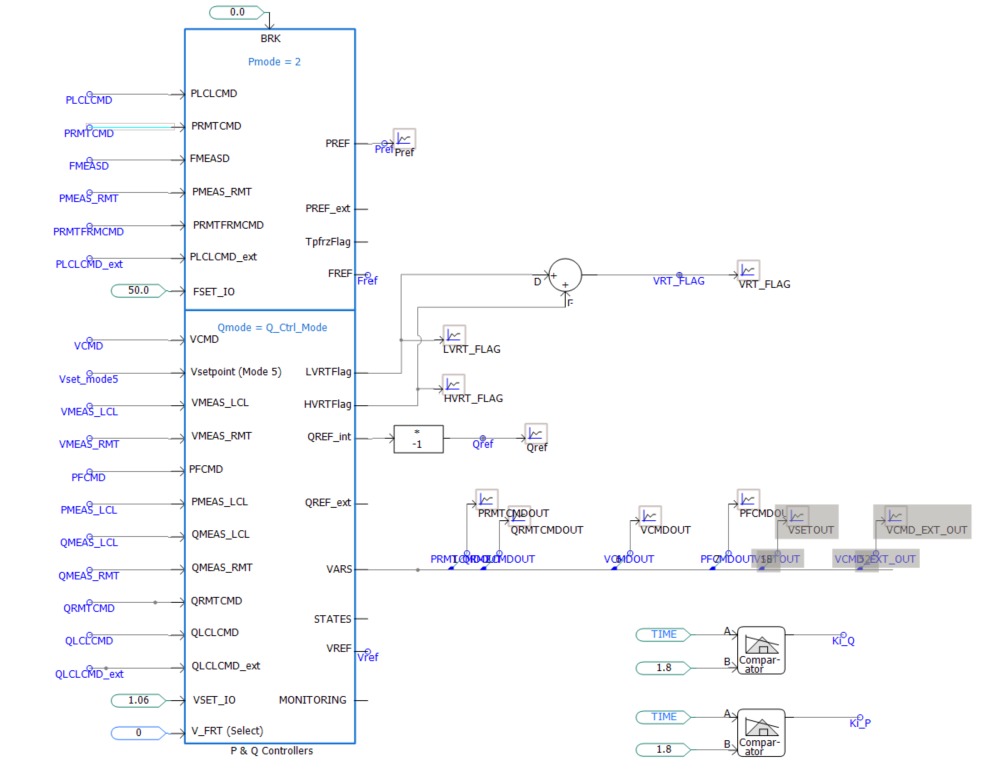
\includegraphics[width=\textwidth]{report-assets/images/ppm-inputs.png}
		\caption{Inputs to the PPM}
		\label{fig:ppm-inputs}
	\end{figure}
		
{
	\thicktablelines
	\begin{longtable}{|C{4cm}|C{2cm}|C{10cm}|} 
		\caption{PPC input set point table}
		\label{tab:ppc-inputs-table}
		\\	
		\toprule
		\rowcolor{tableheaderblue}
		\bfseries \color{white}Parameter & \bfseries \color{white}Type & \bfseries \color{white}Description\\
		\endhead
		\bottomrule \endfoot
		
		\csvreader[
		separator=comma,
		late after line=\\\hline,
		late after last line=,
		before reading={\catcode`\#=12},
		after reading={\catcode`\#=6}
		]%
		{report-assets/ppc_inputs_table.csv} % Update path if needed
		{1=\CSVVariable, 2=\CSVType, 3=\CSVDescription}
		{\CSVVariable & \CSVType & \CSVDescription}
		\\\hline
		
	\end{longtable}
}

	
	\subsection{Simulation with a reduced number of converters and MV auxiliary transformers}
	
	

	To perform simulations with a reduced number of converters, the following parameters needs to be adjusted in each branch by modifying the input to the scaling component as pictured below in Figure \ref{fig:inv-scaling-component}.

	All other parameters of the converter and converter transformer are in pu and will be adjusted automatically.
	
	
	\begin{figure}[H]
		\centering
		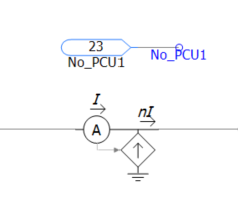
\includegraphics[width=0.3\textwidth]{report-assets/images/inv-scaling-component.png}
		\caption{Converters and Auxiliary transformers scaling component}
		\label{fig:inv-scaling-component}
	\end{figure}
	

	
	
	\subsection{Use of external automation}
	
	A user wanting to apply their own set points from some external module can do so by setting the \$( AUTO_Automation_Mode_Enabled) global substitution to 1, then replacing the top branch of the automation switch with their own automation module, as shown in Figure \ref{fig:ext-auto}. The automation module used should produce a 50 element list of signals to be applied to the 50 elements in the UNMERGER list. If this is not practical, the user can take the signals they want to control out of the UNMERGER list and connect them to their own automation as required without using the MERGER and UNMERGER elements.
	
	\bfseries{IMPORTANT: The disabled ‘Pallet’ block is used by Grid-Link for automation and should not be enabled unless directed to do so by Grid-Link as it will cause PSCAD to error unless other infrastructure is present. A 50 element array of ‘1’s is assigned to this branch instead as it is assumed that most users will not manipulate this section.}


	\begin{figure}[H]
		\centering
		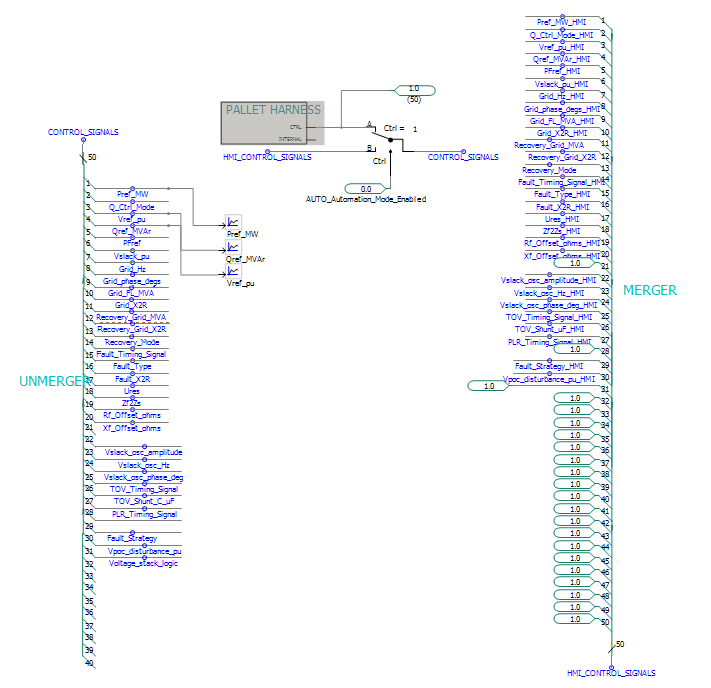
\includegraphics[width=0.8\textwidth]{report-assets/images/ext-auto-new.png}
		\caption{Use of external automation}
		\label{fig:ext-auto}
	\end{figure}

	
	\chapter*{Acronyms}
\begin{acronym}%[JSONP]\itemsep0pt
	\acro{AAS}{Automatic Access Standard}
	\acro{AEMO}{Australian Energy Market Operator}
	\acro{VSL}{Voltage Stackable Logic}
	\acro{AGC}{Automatic Generation Control}
	\acro{AVR}{Automatic Voltage Regulator}
	\acro{BESS}{Battery Energy Storage System}
	\acro{BOP}{Balance Of Plant}
	\acro{CGBESS}{Clements Gap BESS}
	\acro{Heywood BESS}{Heywood Battery Energy Storage System}	
	\acro{CSR}{Connection Studies Report}
	\acro{CT}{Current Transformer}
	\acro{CUO}{Continuous Uninterrupted Operation}
	\acro{HV}{High Voltage}
	\acro{DMAT}{Dynamic Model Acceptance Test}
	\acro{DYR}{PSSE Dynamics Data File}
	\acro{EMT}{Electromagnetic Transients}
	\acro{FIA}{Full Impact Assessment}
	\acro{FRT}{Fault Ride-Through}
	\acro{GPS}{Generator Performance Standards}
	\acro{HVRT}{High Voltage Ride-Through}
	\acro{LV}{Low Voltage}
	\acro{LVRT}{Low Voltage Ride-Through}
	\acro{MV}{Medium Voltage}
	\acro{NEM}{National Electricity Market}
	\acro{NSP}{Network Service Provider}
	\acro{OEM}{Original Equipment Manufacturer}
	\acro{OFRT}{Over-Frequency Ride-Through}
	\acro{OLTC}{On-Load Tap Changer}
	\acro{OPDMS}{Operations and Planning Data Management System}
	\acro{OVRT}{Over-Voltage Ride-Through}
	\acro{PLL}{Phase-Locked Loop}
	\acro{PLR}{Partial Load Rejection}
	\acro{PPC}{Power Plant Controller}
	\acro{PPM}{Power Plant Manager}
	\acro{RoCoF}{Rate of Change of Frequency}
	\acro{RMS}{Root Mean Square}
	\acro{RMU}{Ring Main Unit}
	\acro{RUG}{Releasable User Guide}
	\acro{S5251}{Reactive Power Capability}
	\acro{S5254}{Generating System Response to Voltage Disturbances}
	\acro{SCR}{Short Circuit Ratio}
	\acro{SMIB}{Single Machine, Infinite Bus}
	\acro{SLD}{Single Line Diagram}
	\acro{TOV}{Temporary Over-Voltage}
	\acro{UFRT}{Under-Frequency Ride-Through}
	\acro{UVRT}{Under-Voltage Ride-Through}
	\acro{VCS}{Voltage Control Strategy}
	\acro{WAN}{Wide Area Network}
	\acro{WF}{Wind Farm}
	\acro{VOIP}{Voice Over Internet Protocol}
	\acro{VRR}{Voltage Regulation Relay}
	\acro{VT}{Voltage Transformer}
\end{acronym}
	
	\chapter{Appendix A: Model parameters}
	

	
	
	\section{Aggregated transformer parameters}
	
	
			
	% Aggregate transformer parameter table
	{%
		\thicktablelines
		\begin{longtable}{|C{6cm}|C{6cm}|} 
			\caption{Grid transformer parameters}
			\label{tab:aggr-transformer}
			\\	
			\toprule
			
			\rowcolor{tableheaderblue}
			\bfseries \color{white}Parameter & \bfseries \color{white}Value
			\endhead
			\bottomrule \endfoot
			\csvreader[
			separator=comma,
			late after line=\\\hline,
			late after last line=,
			before reading={\catcode`\#=12},
			after reading={\catcode`\#=6}]%
			{report-assets/GTX.csv}{1=\COLA,2=\COLB}{\COLA & \COLB}
			\\\hline
		\end{longtable}
	}
	
	{%
		\thicktablelines
		\begin{longtable}{|C{6cm}|C{6cm}|} 
			\caption{Inverter transformer parameters (aggregated)}
			\label{tab:inv-transformer}
			\\	
			\toprule
			
			\rowcolor{tableheaderblue}
			\bfseries \color{white}Parameter & \bfseries \color{white}Value
			\endhead
			\bottomrule \endfoot
			\csvreader[
			separator=comma,
			late after line=\\\hline,
			late after last line=,
			before reading={\catcode`\#=12},
			after reading={\catcode`\#=6}]%
			{report-assets/INVTX.csv}{1=\COLA,2=\COLB}{\COLA & \COLB}
			\\\hline
		\end{longtable}
	}

	\section{275kV Underground Cable}

	
% Lines and Cable parameters for Cable from HVTX to POC
{%
	\thicktablelines
	\begin{longtable}{|C{2cm}|C{3cm}|C{6cm}|C{1cm}|C{4cm}|} 
		\caption{Lines and Cable parameters for Cable connecting from HV Transformer to POC (based on 100MVA and 275kV)}
		\label{tab:line-cables-275kV}
		\\	
		\toprule
		
		\rowcolor{tableheaderblue}
		\bfseries \color{white}CableGroup & \bfseries \color{white}Parameter & \bfseries \color{white}Description & \bfseries \color{white}Units & \bfseries \color{white}HEYWOODBESS \\
		\endhead
		\bottomrule \endfoot
		\csvreader[
		separator=comma,
		late after line=\\\hline,
		late after last line=,
		before reading={\catcode`\#=12},
		after reading={\catcode`\#=6}]%
		{report-assets/lines-cables-parameters-275kV.csv}{1=\CSVCableGroup,2=\CSVParameter,3=\CSVDescription,4=\CSVUnits,5=\CSVHEYWOODBESS}{\CSVCableGroup & \CSVParameter & \CSVDescription & \CSVUnits & \CSVHEYWOODBESS }
		\\\hline
	\end{longtable}
}

	\section{33kV reticulation}
	

	
	
	
	
	% Lines and Cable parameters for Cable connecting to Main Transformer
	{%
		\thicktablelines
		\begin{longtable}{|C{2cm}|C{3cm}|C{6cm}|C{1cm}|C{4cm}|} 
			\caption{Lines and Cable parameters for Cable connecting from 33kV switchboard to HV transformer (based on 100MVA and 33kV)}
			\label{tab:line-cables-inv}
			\\	
			\toprule
			
			\rowcolor{tableheaderblue}
			\bfseries \color{white}CableGroup & \bfseries \color{white}Parameter & \bfseries \color{white}Description & \bfseries \color{white}Units & \bfseries \color{white}HEYWOODBESS \\
			\endhead
			\bottomrule \endfoot
			\csvreader[
			separator=comma,
			late after line=\\\hline,
			late after last line=,
			before reading={\catcode`\#=12},
			after reading={\catcode`\#=6}]%
			{report-assets/lines-cables-parameters-MainTX.csv}{1=\CSVCableGroup,2=\CSVParameter,3=\CSVDescription,4=\CSVUnits,5=\CSVHEYWOODBESS}{\CSVCableGroup & \CSVParameter & \CSVDescription & \CSVUnits & \CSVHEYWOODBESS }
			\\\hline
		\end{longtable}
	}
	
	% Lines and Cable parameters for Cable connecting from MVTX to 33kV switchroom
	{%
		\thicktablelines
		\begin{longtable}{|C{2cm}|C{3cm}|C{6cm}|C{1cm}|C{4cm}|} 
			\caption{Lines and Cable parameters for Cable connecting from MV transformers to 33kV switchboard(based on 100MVA and 33kV)}
			\label{tab:line-cables-inv}
			\\	
			\toprule
			
			\rowcolor{tableheaderblue}
			\bfseries \color{white}CableGroup & \bfseries \color{white}Parameter & \bfseries \color{white}Description & \bfseries \color{white}Units & \bfseries \color{white}HEYWOODBESS \\
			\endhead
			\bottomrule \endfoot
			\csvreader[
			separator=comma,
			late after line=\\\hline,
			late after last line=,
			before reading={\catcode`\#=12},
			after reading={\catcode`\#=6}]%
			{report-assets/lines-cables-parameters-Inv.csv}{1=\CSVCableGroup,2=\CSVParameter,3=\CSVDescription,4=\CSVUnits,5=\CSVHEYWOODBESS}{\CSVCableGroup & \CSVParameter & \CSVDescription & \CSVUnits & \CSVHEYWOODBESS }
			\\\hline
		\end{longtable}
	}
	
		%
	{	
		\thicktablelines
		\begin{longtable}{|C{5cm}|C{4cm}|C{2cm}|}
			\caption{System strength conditions}
			\label{tab:fault-details} \\
			\toprule
			\rowcolor{tableheaderblue}
			\bfseries \color{white}Condition & \bfseries \color{white}Fault Level (MVA) & \bfseries \color{white}X/R Ratio \\
			\endhead
			\bottomrule \endfoot
			\csvreader[
			late after line=\\\hline,
			late after last line=,
			before reading={\catcode`\#=12},
			after reading={\catcode`\#=6}]% 
			{report-assets/fault-details.csv}{1=\CSVParameter,2=\CSVValue,3=\CSVUnit}{\CSVParameter & \CSVValue & \CSVUnit}
			\\\hline
		\end{longtable}
	}	

	\section{Converters}
	
	\lstinputlisting{report-assets/CfgFile57.txt}
	
	\section{Power Plant Control}

		\begin{figure}[H]
		\centering
		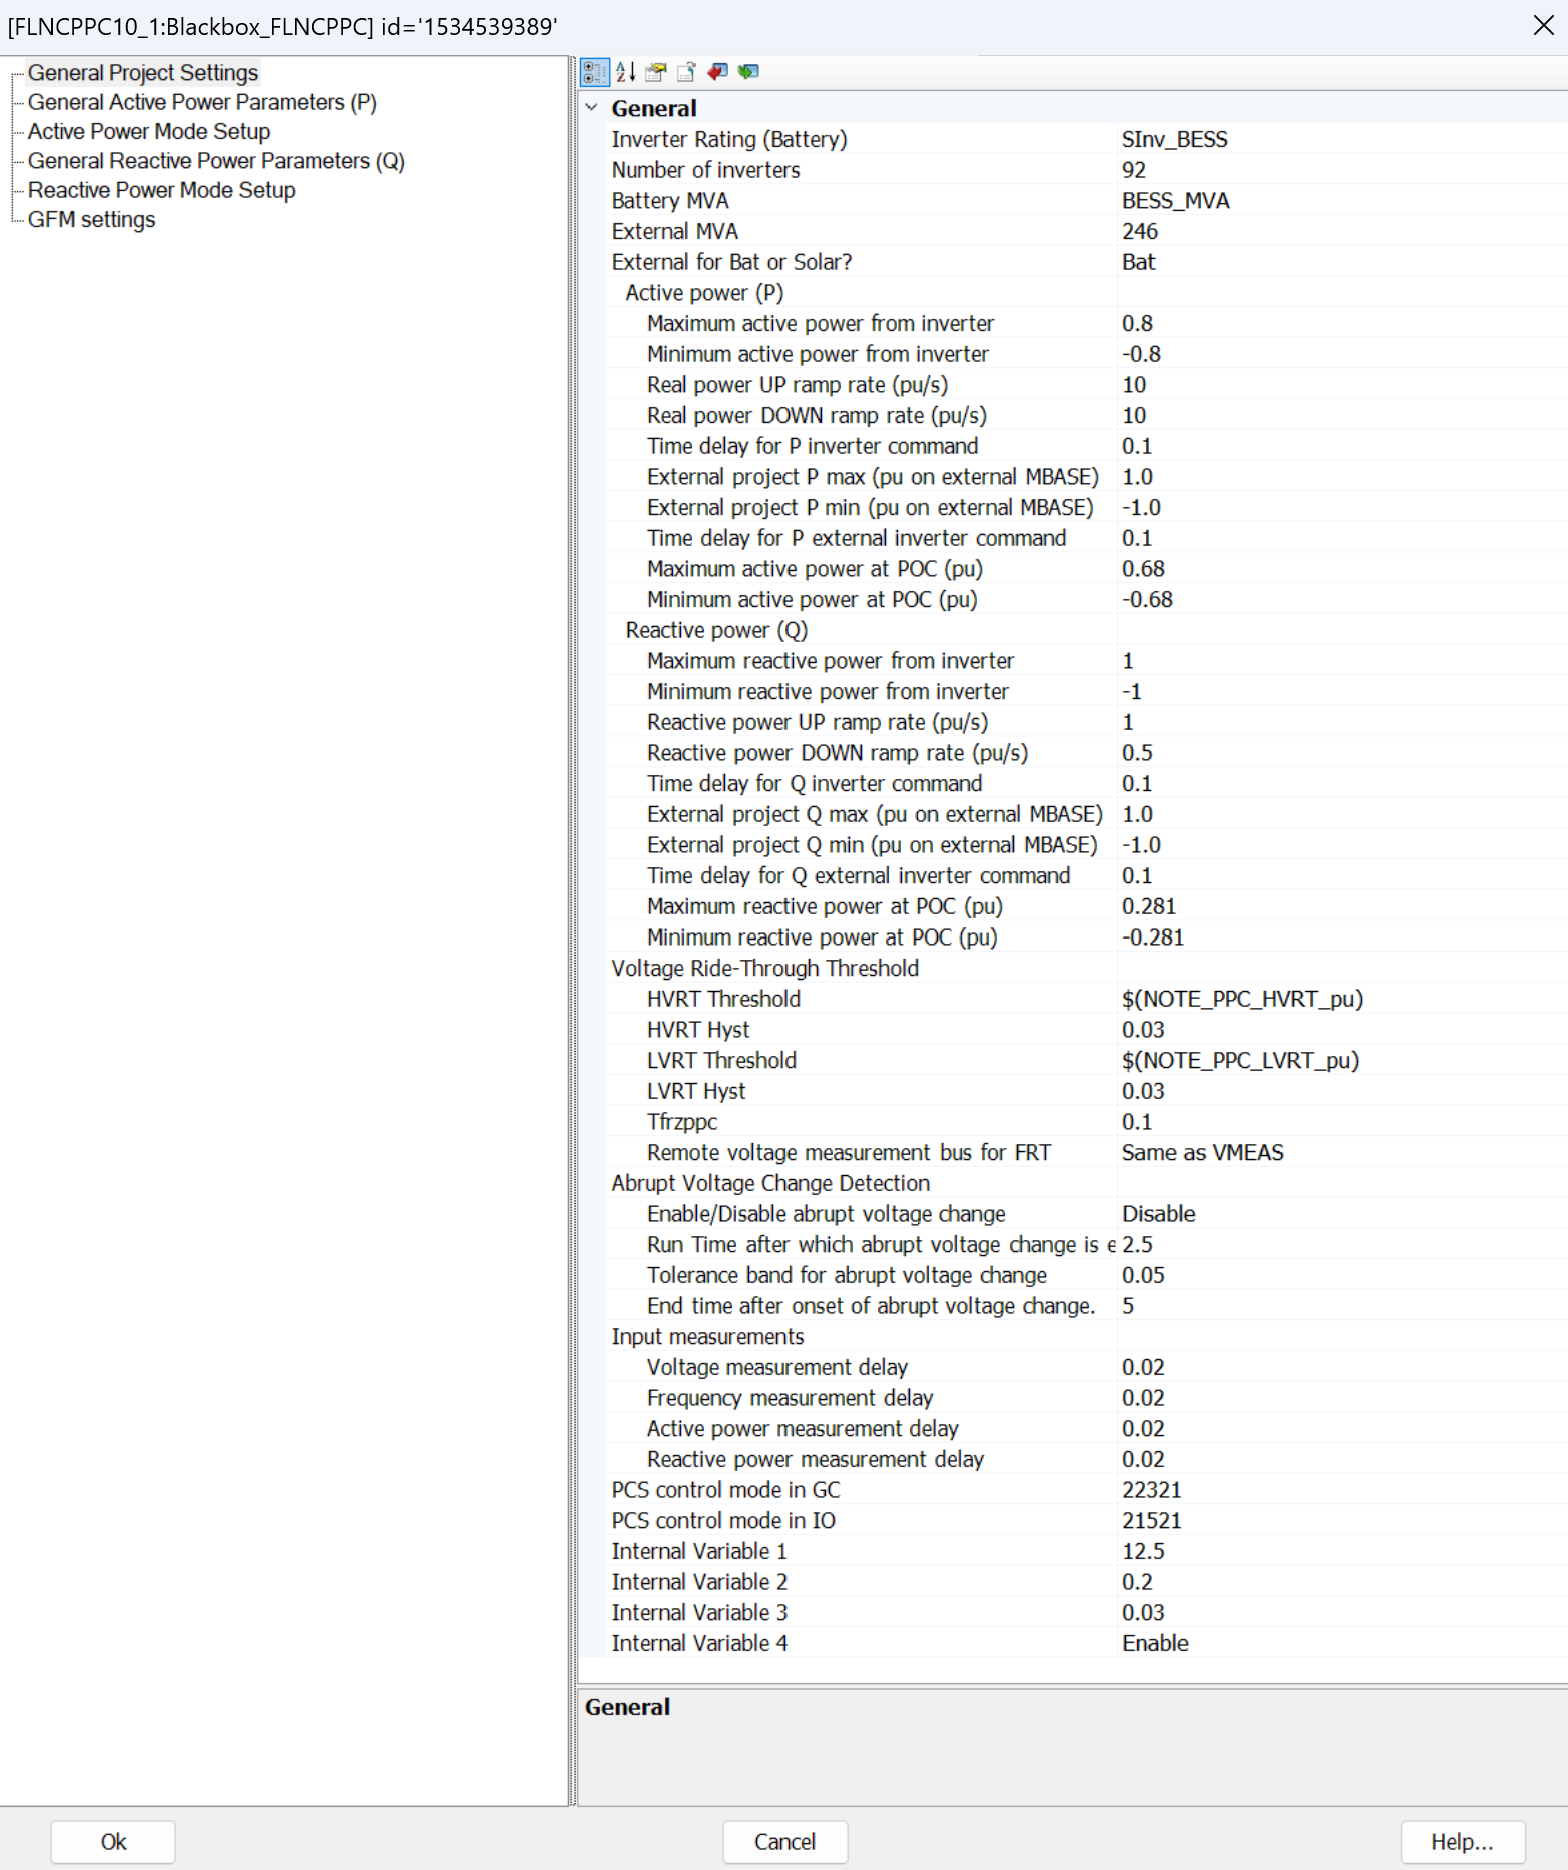
\includegraphics[width=\textwidth]{report-assets/images/General Project Settings.png}
		\caption{General Project Settings}
		\label{fig:General Project Settings}
	\end{figure}
	
		\begin{figure}[H]
		\centering
		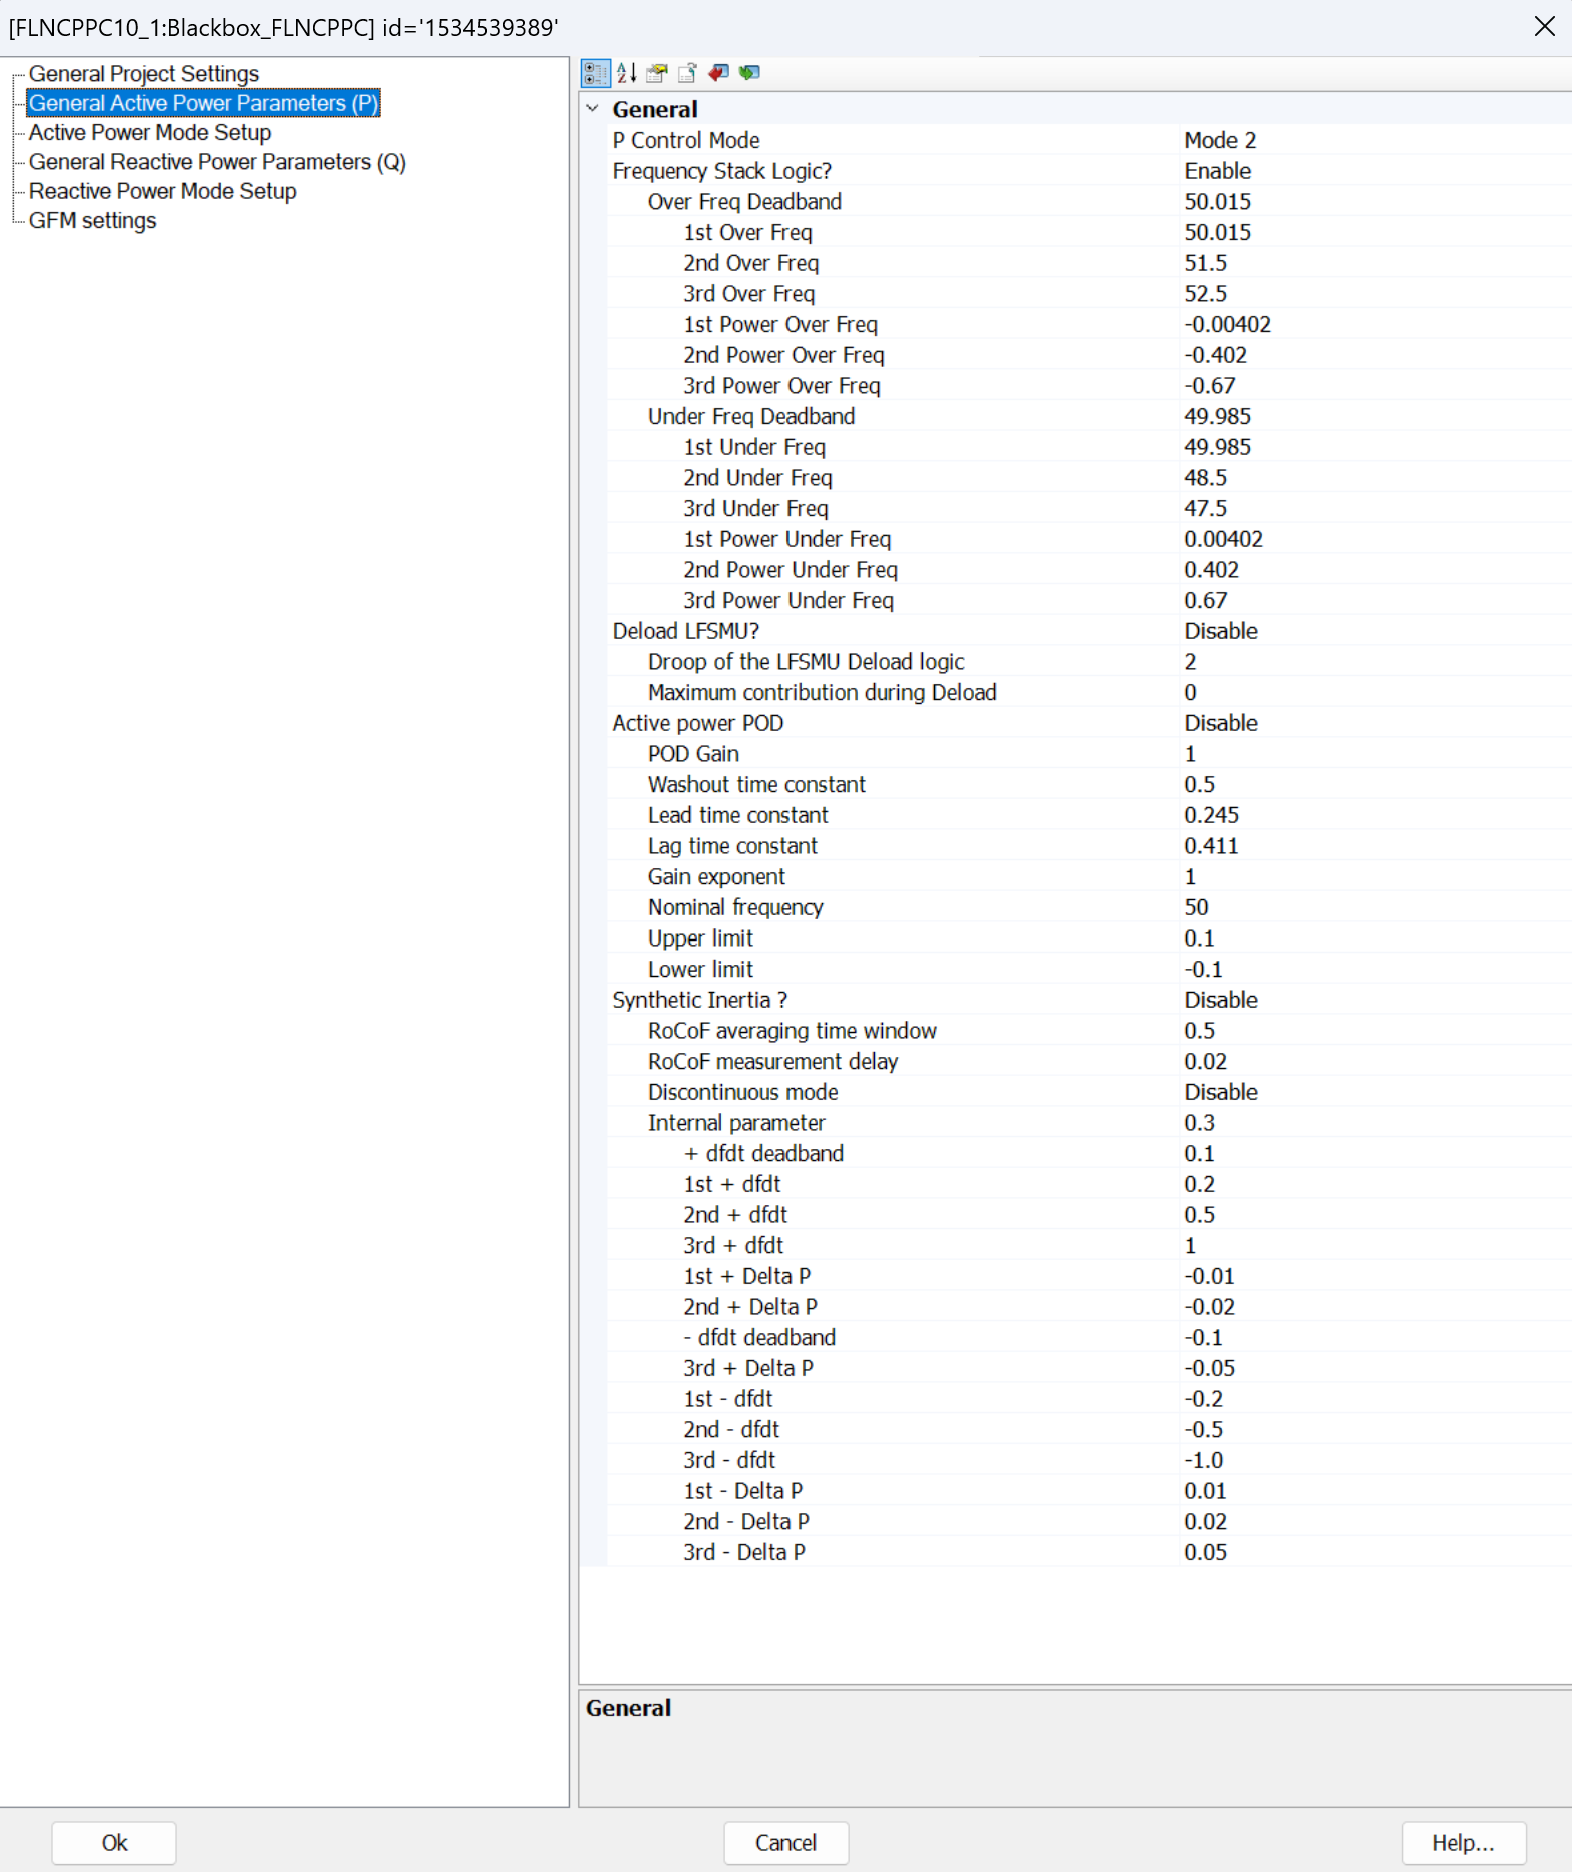
\includegraphics[width=\textwidth]{report-assets/images/General Active Power Parameters (P).png}
		\caption{General Active Power Parameters (P)}
		\label{fig:General Active Power Parameters (P)}
	\end{figure}
	
		\begin{figure}[H]
		\centering
		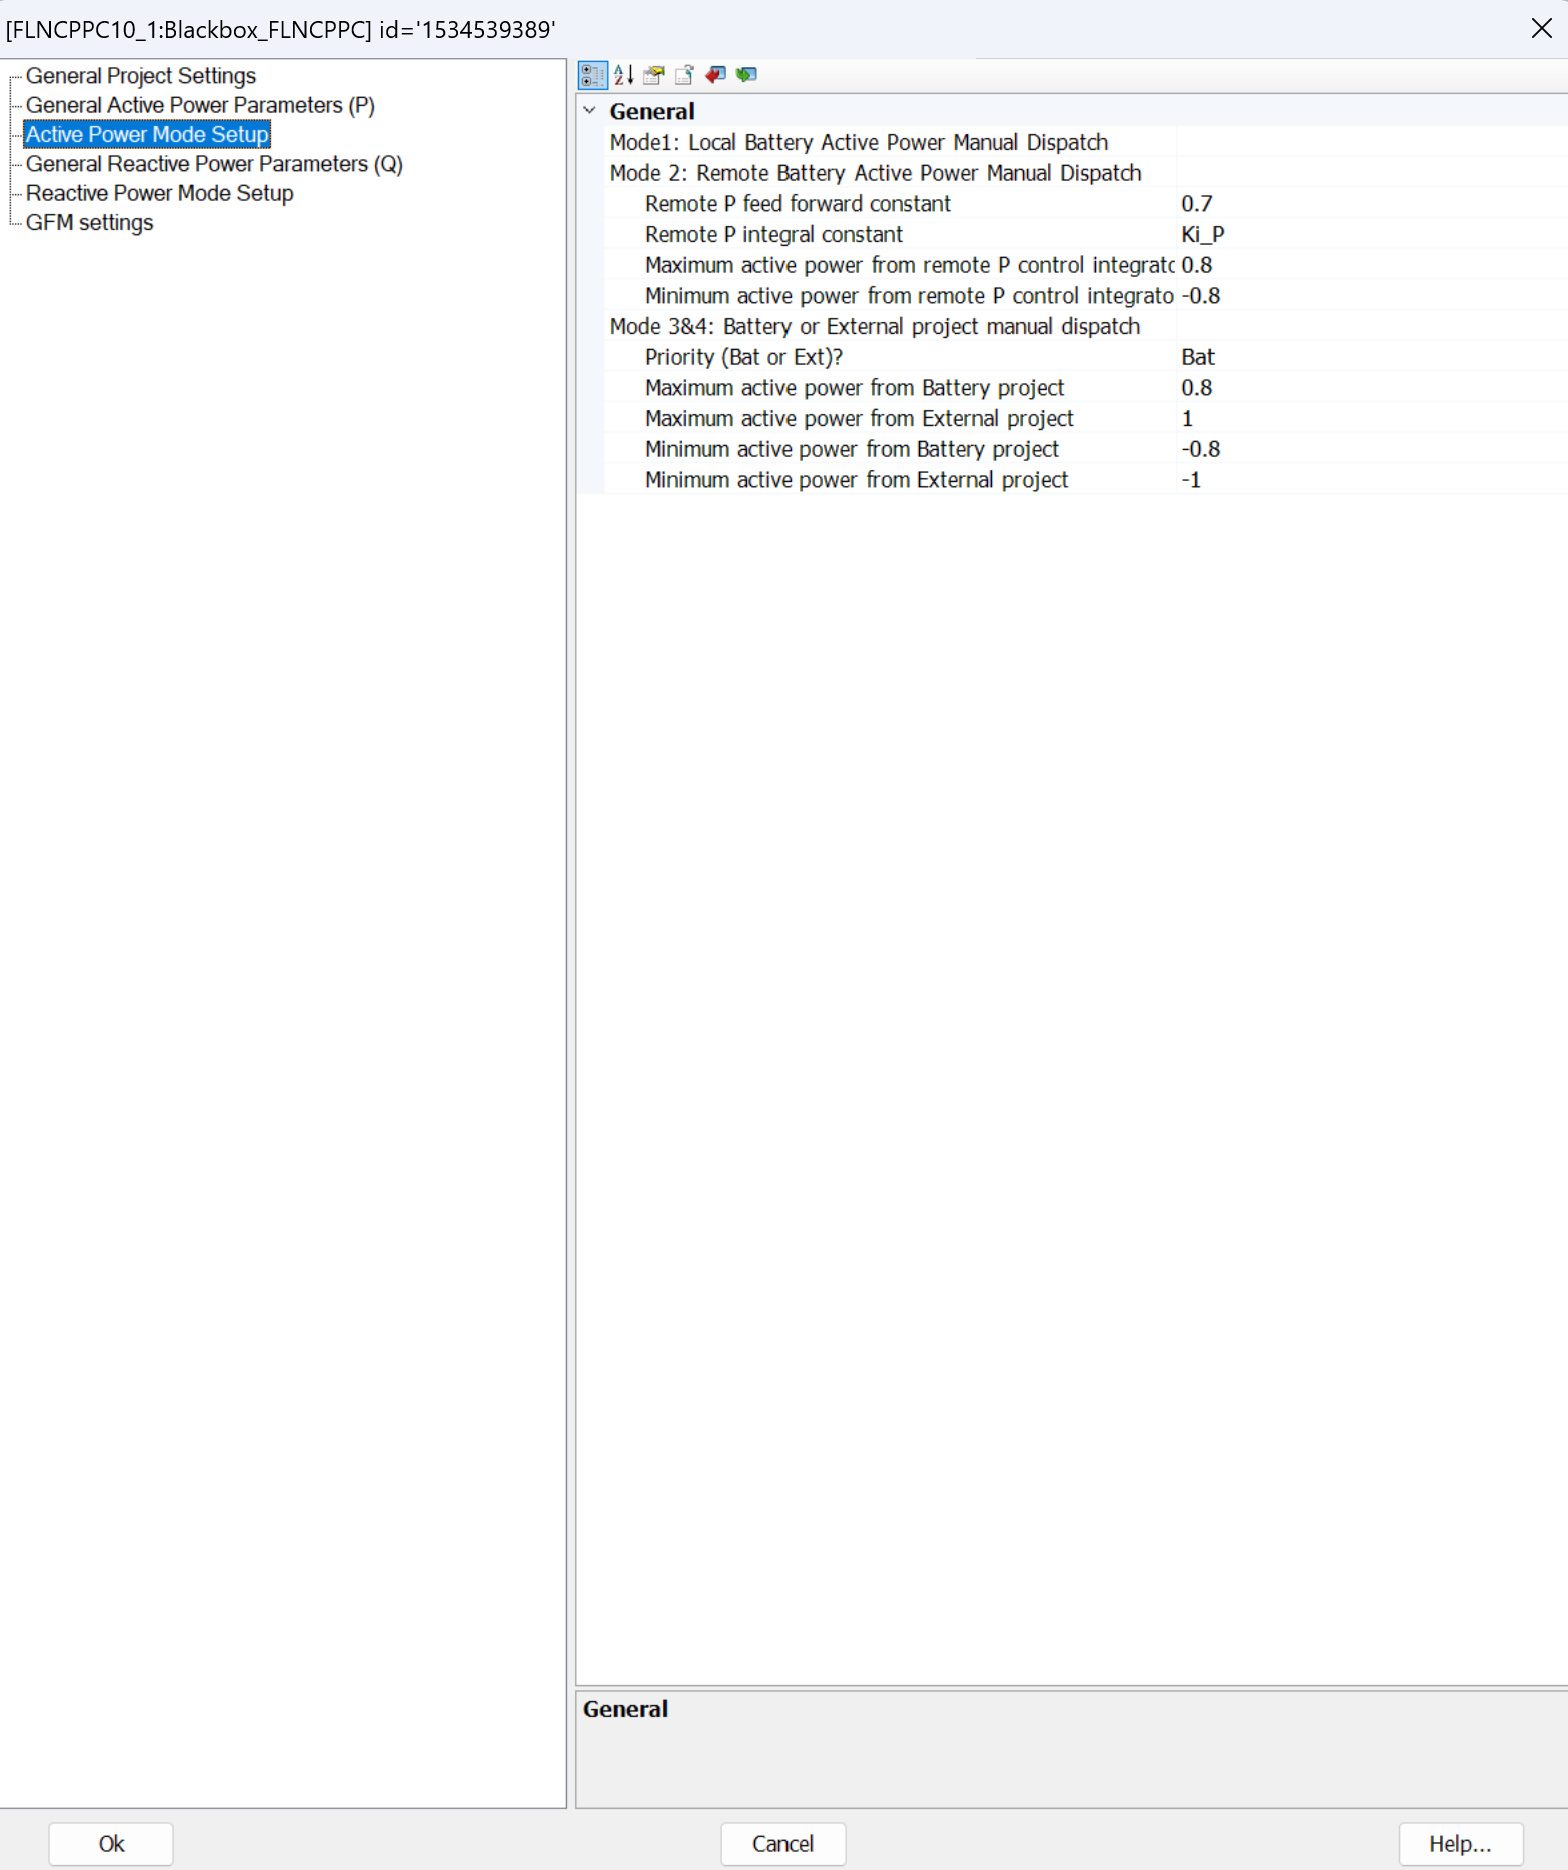
\includegraphics[width=\textwidth]{report-assets/images/Active Power Mode Setup.png}
		\caption{Active Power Mode Setup}
		\label{fig:Active Power Mode Setup}
	\end{figure}
	
		\begin{figure}[H]
		\centering
		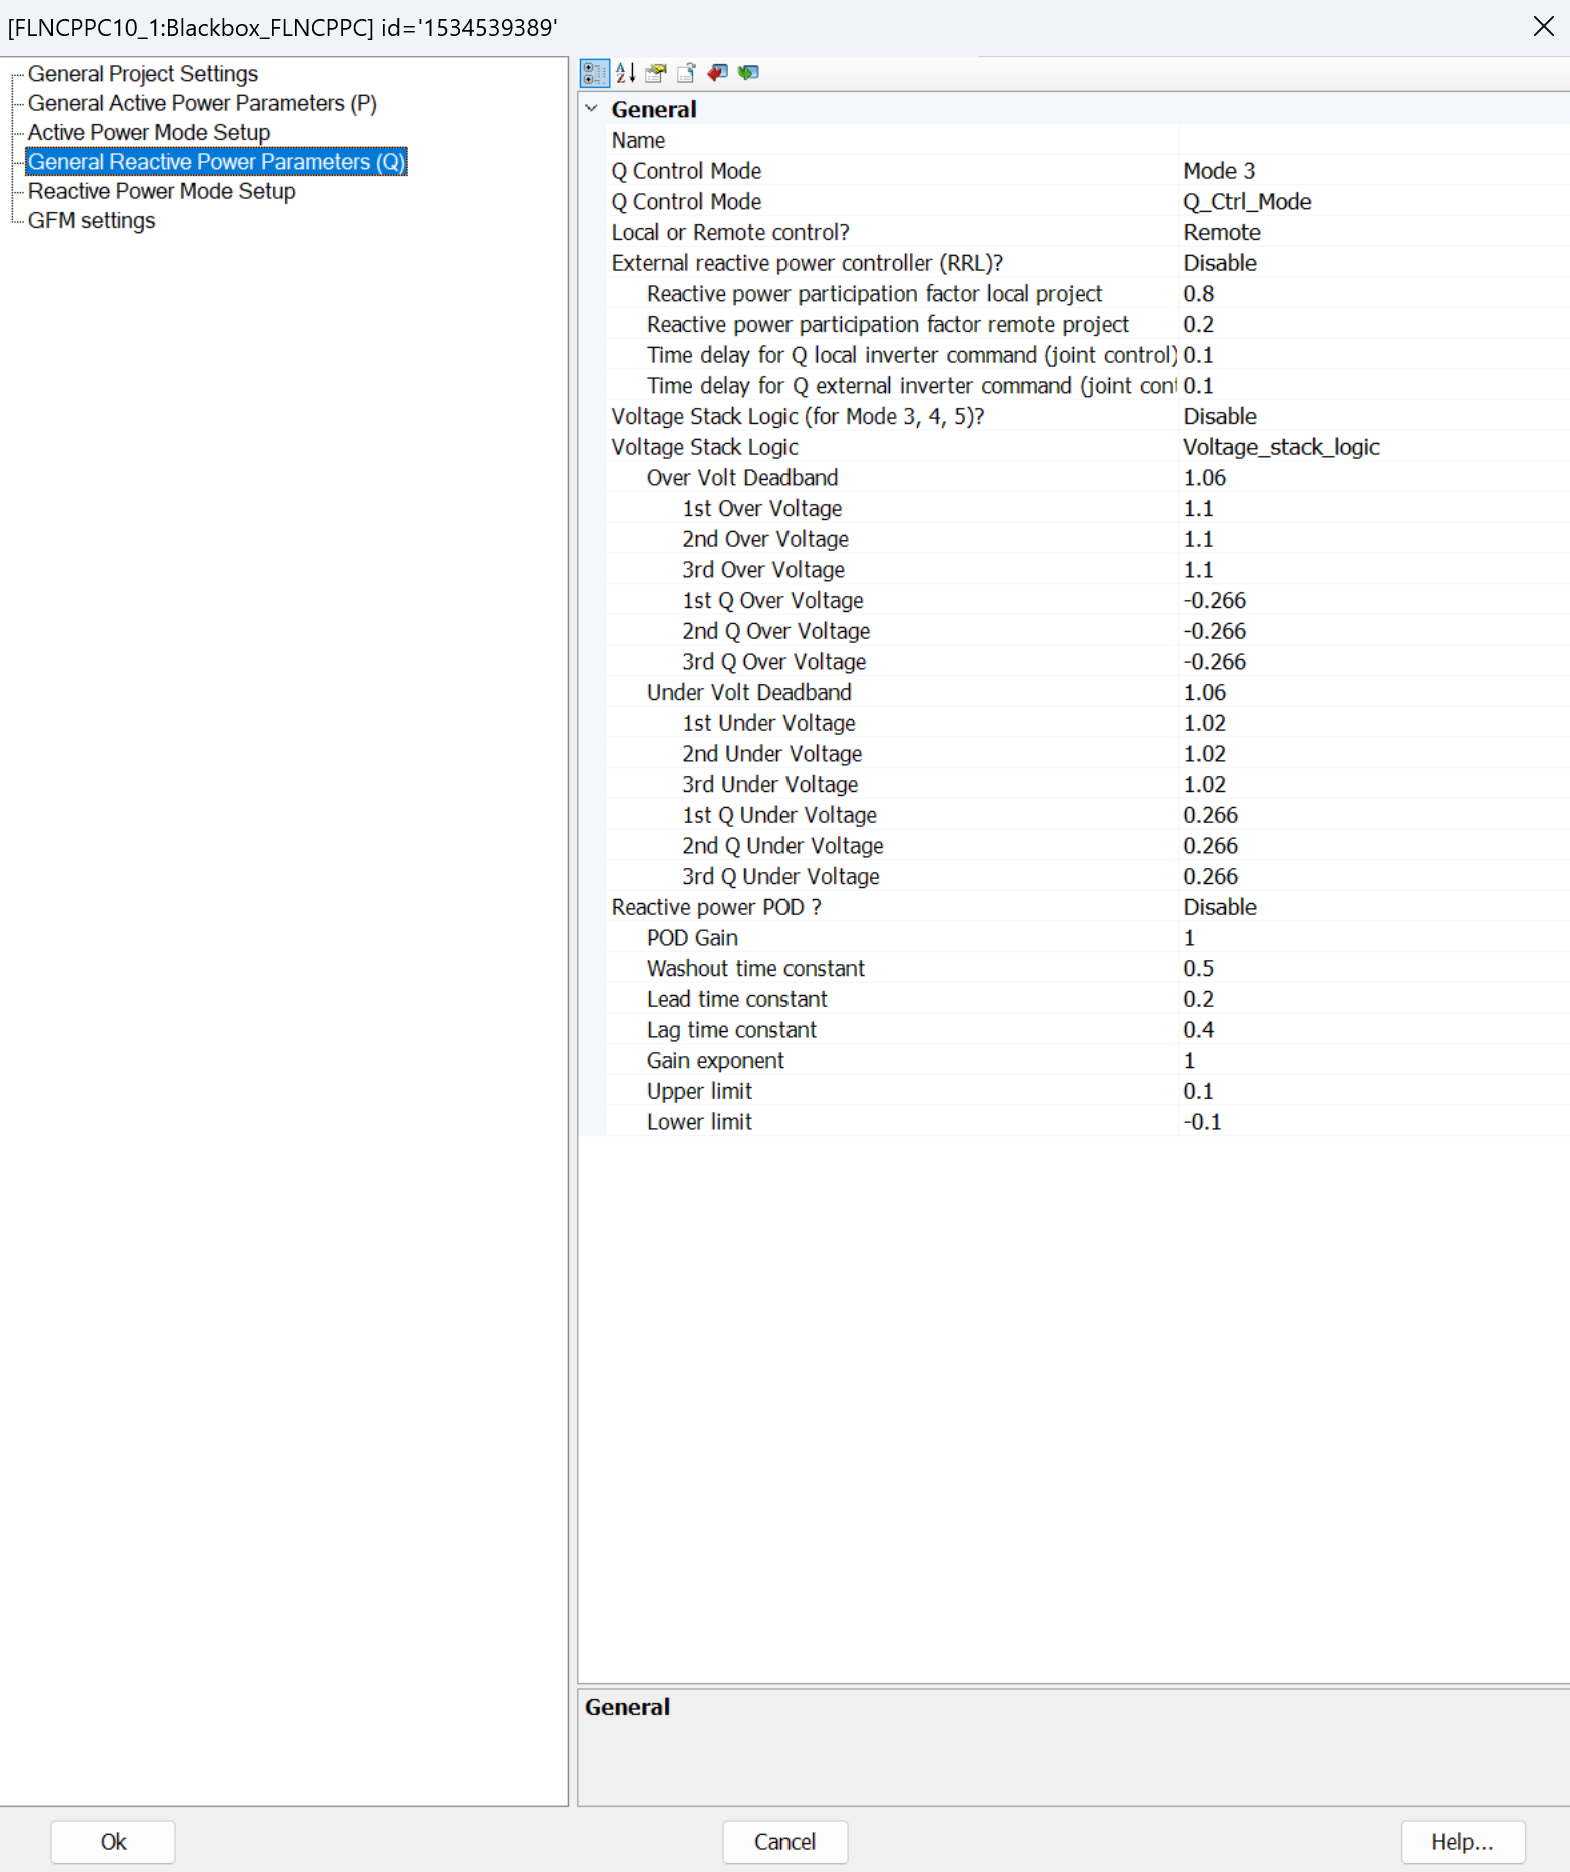
\includegraphics[width=\textwidth]{report-assets/images/General Reactive Power Parameters (Q).png}
		\caption{General Reactive Power Parameters (Q)}
		\label{fig:General Reactive Power Parameters (Q)}
	\end{figure}
	
		\begin{figure}[H]
		\centering
		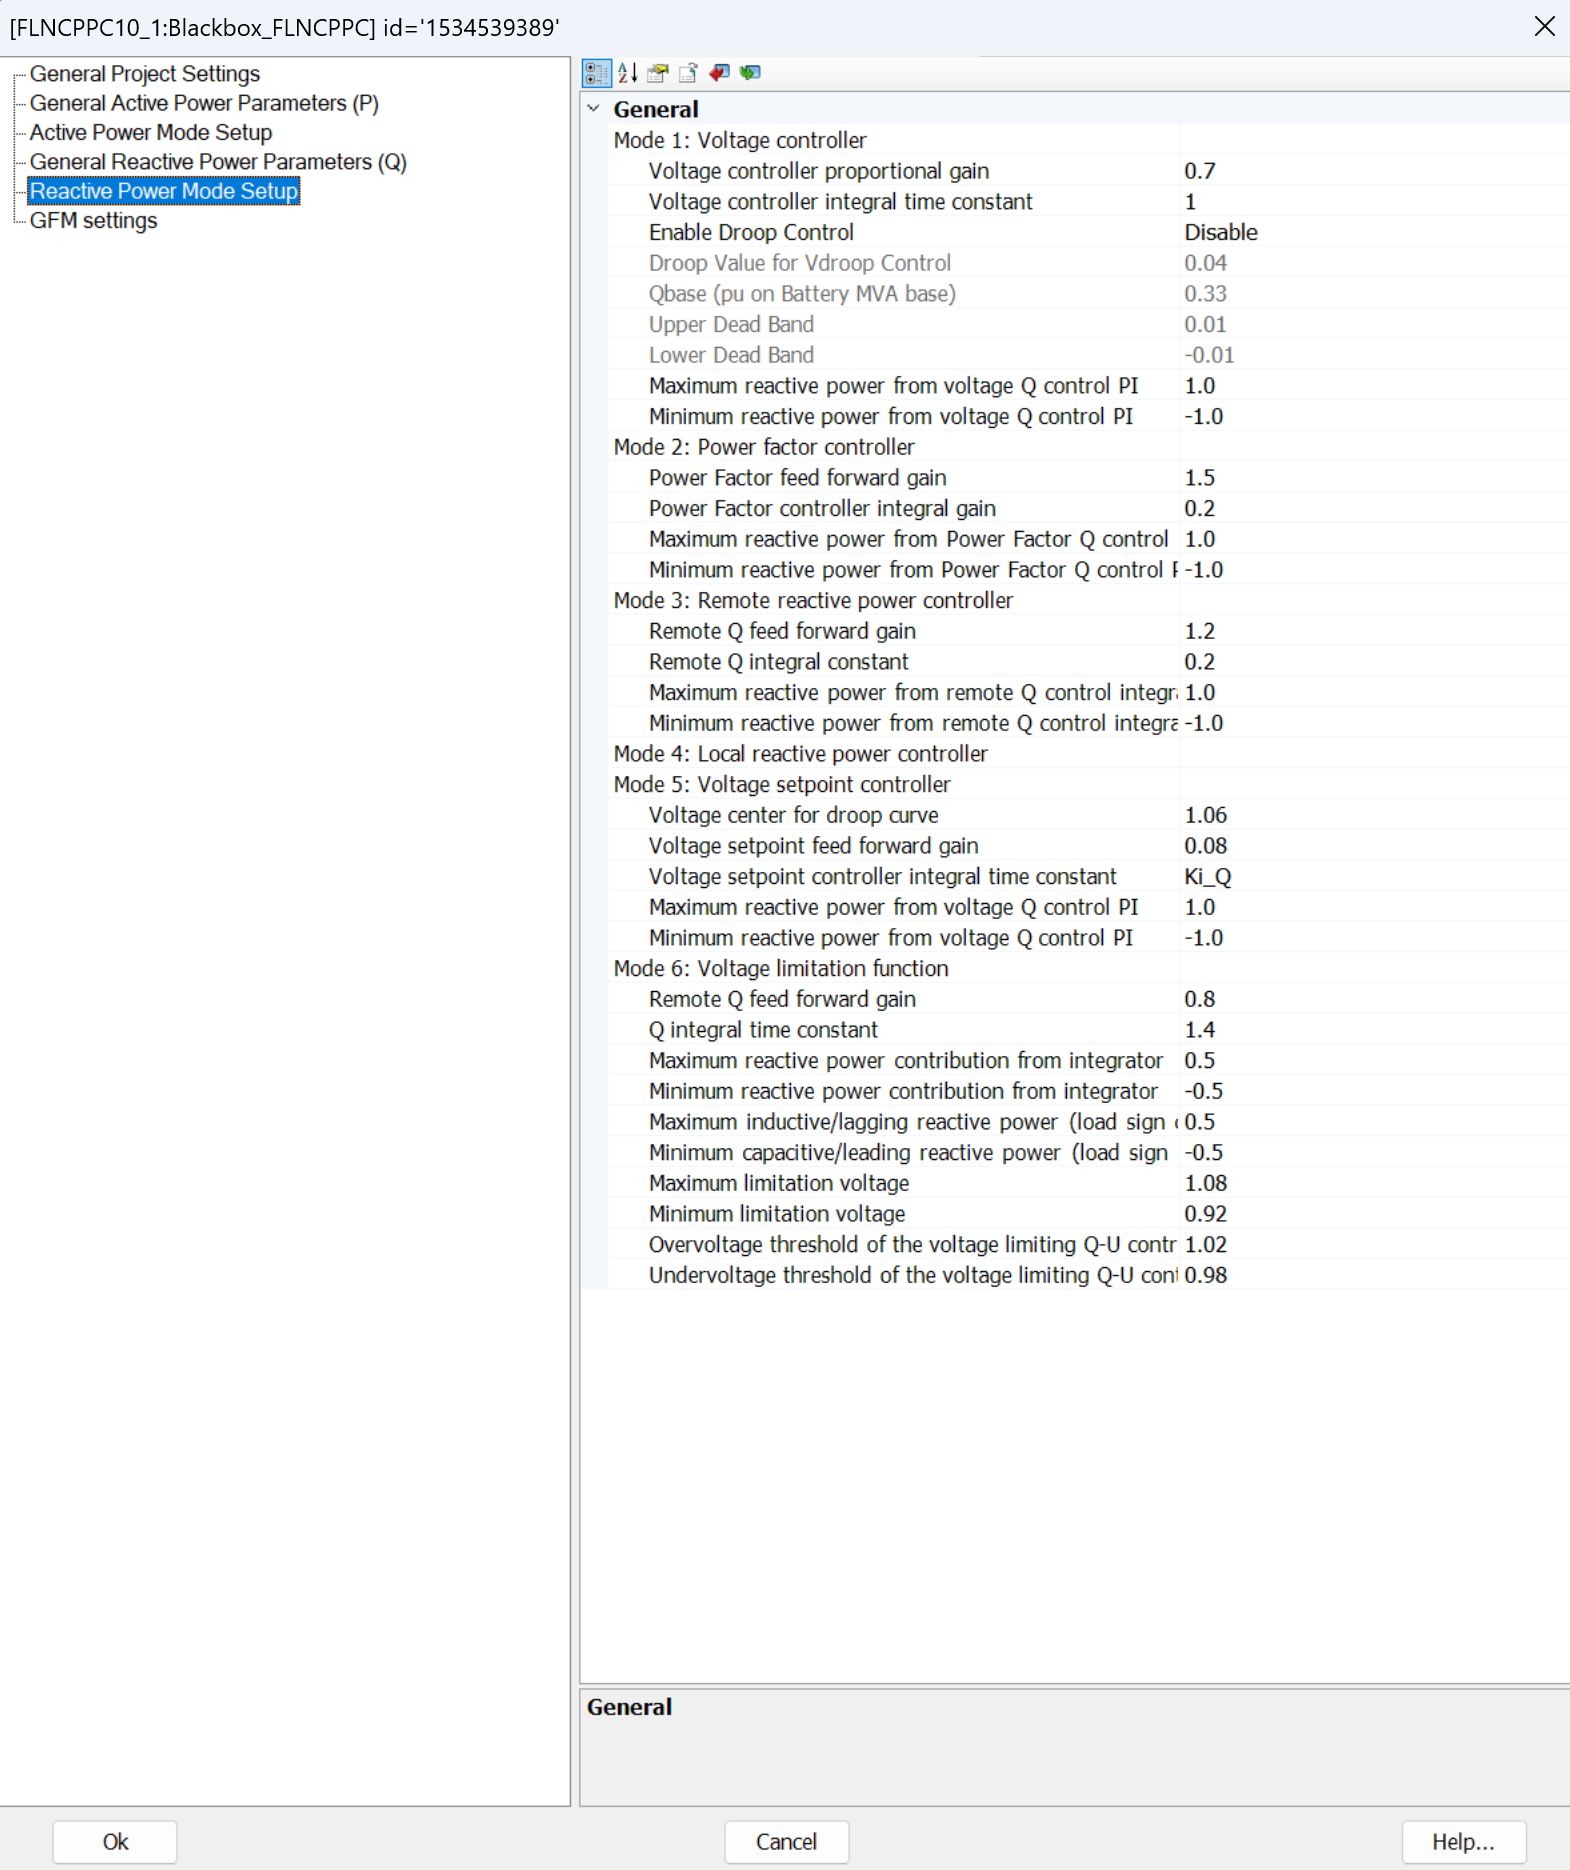
\includegraphics[width=\textwidth]{report-assets/images/Reactive Power Mode Setup.png}
		\caption{Reactive Power Mode Setup}
		\label{fig:Reactive Power Mode Setup}
	\end{figure}
	
		\begin{figure}[H]
		\centering
		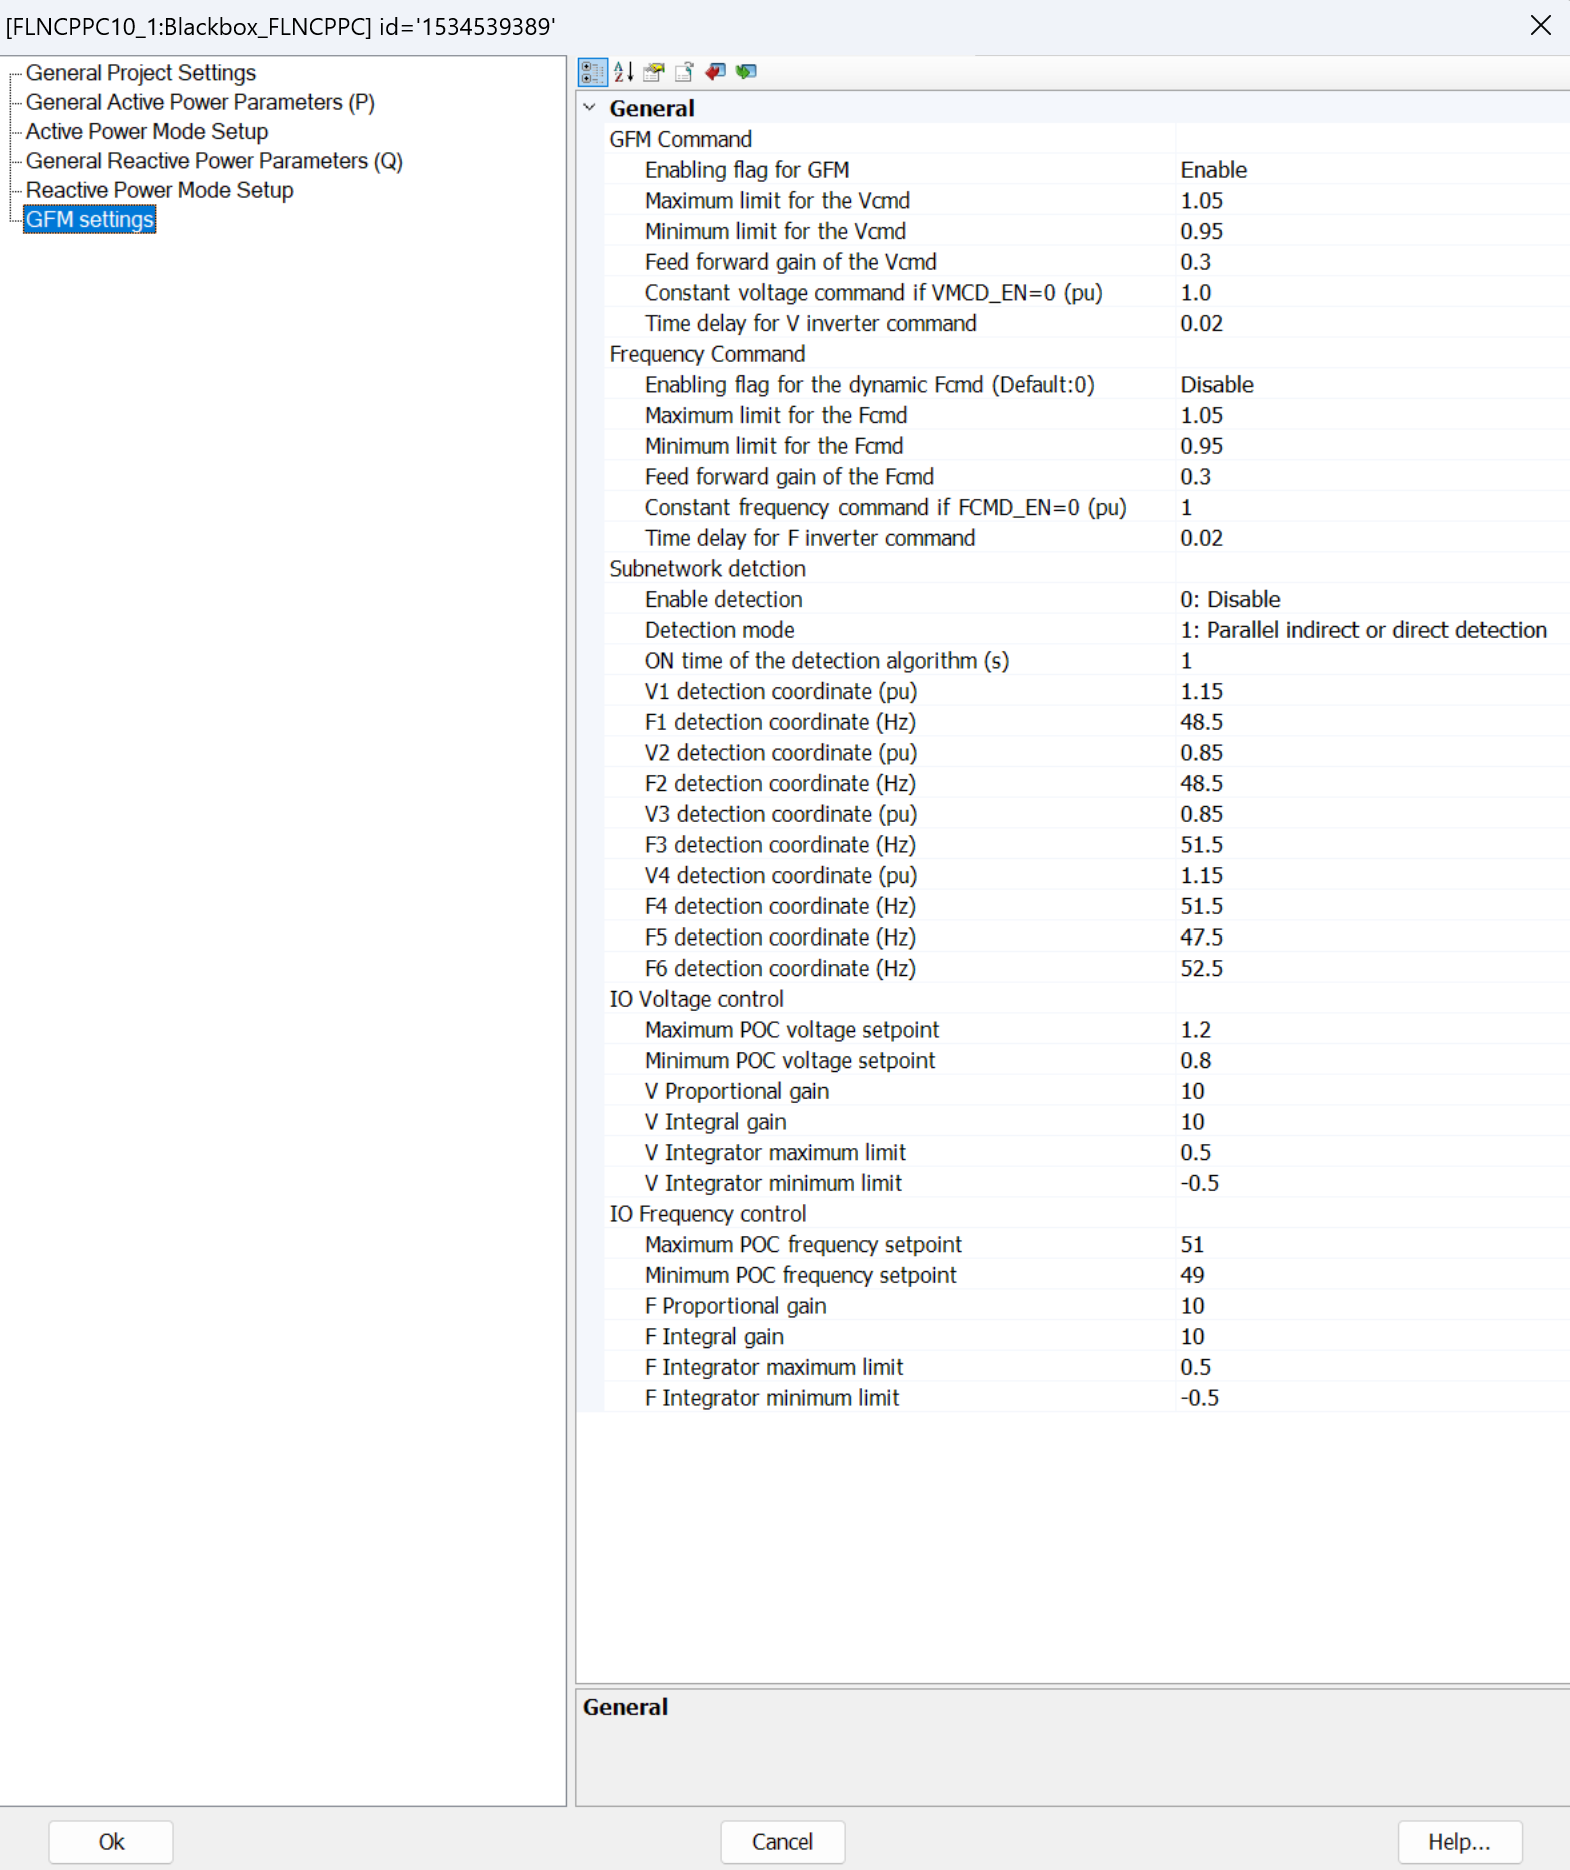
\includegraphics[width=\textwidth]{report-assets/images/GFM settings.png}
		\caption{GFM settings}
		\label{fig:GFM settings}
	\end{figure}
	
	
	\makebackpage
\end{document}